\documentclass[]{beamer}
% \usecolortheme[named=OliveGreen]{structure}
%\usetheme{Boadilla}
% \usetheme{Madrid}
%\usetheme{Malmoe} 
%\usetheme{Singapore} 
%\usetheme{Warsaw}
%\usetheme{Copenhagen}
%\usetheme{Frankfurt}
% \setbeamercolor{structure}{fg=OliveGreen!50!black} 
%\usecolortheme[named=OliveGreen]{structure} 
%muda a cor do slide


  %  Bergen, Berkeley, Berlin, Boadilla, Copenhagen, Darmstadt,
  % Dresden, Frankfurt, Goettingen, Hannover, Ilmenau, JuanLesPins,
  % Luebeck, Madrid, Malmoe, Marburg, Montpellier, PaloAlto, Pittsburgh,
  % Rochester, Singapore, Szeged, Warsaw, boxes, default.

%\usecolortheme[named=OliverGreen]{structure} 
%muda a cor do slide
\usepackage{multimedia}
\usepackage{amsmath,amssymb}
\usepackage[brazil]{varioref}
\usepackage[english,brazil]{babel}
% \usepackage[latin1]{inputenc}
\usepackage[T1]{fontenc}
\usepackage{graphicx}
\usepackage{subfig}
\usepackage{listings}
\usepackage{url}
\usepackage{colortbl}
\usepackage{ragged2e}

\usepackage{lmodern}
\usetheme{Madrid}
\colorlet{beamer@blendedblue}{green!50!black}

\title[Atividade Avaliativa da Aula 3]{\textit{Transformação de Intensidade e Filtragem Espacial}}
\author[Jônatas, Nayana, Sérgio]{Jônatas Mendes, Nayana Nery, Sérgio Pedrosa}
\institute[IFPB]{Instituto Federal de Educação, Ciência e Tecnologia da Paraíba - IFPB\\
 Programa de Pós-Graduação em Engenharia Elétrica - PPGEE\\
 Disciplina: Processamento Digital de Imagens\\
 Professor: Dr. Carlos Danilo M. Regis
}
  
 \logo{
\includegraphics[height=1.2cm]{Imagens/ifpb-1.png}} 
 
\newtheorem{teorema}{Teorema}
\newtheorem{lema}{Lema}
\newtheorem{prova}{Prova}
\newtheorem{definicao}{Definição}
\newtheorem{proposicao}{Proposição}
\newtheorem{corolario}{Corolário}
  
\begin{document}

\frame{\titlepage}

\section[Sumário]{}
\frame{\tableofcontents}

\section{Introdução}

\begin{frame}{Introdução}

\begin{itemize}
    \item Informações ocultas;
    \item Segmentação;
    \item Não proposital: Correção \textit{Gamma} e binarização;
    \item Proposital: LSB e MSB.
\end{itemize}

\end{frame}

\section{Fundamentação Teórica}

\subsection{Correção \textit{Gamma}}

\begin{frame}{Fundamentação Teórica - Correção \textit{Gamma}}
    \begin{figure}
        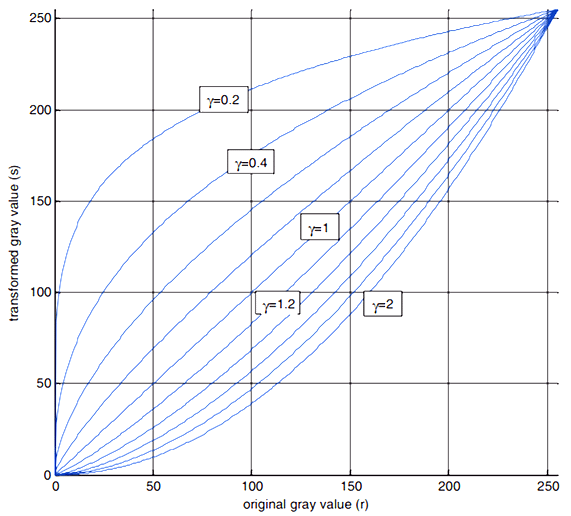
\includegraphics[scale=0.4]{Imagens/Transfer-characteristics-for-power-law-intensity-transformation.png}
    \end{figure}  
\end{frame}

\subsection{Binarização}

\begin{frame}{Fundamentação Teórica - Binarização}
    \begin{columns}
            \column{0.3\textwidth}
            \begin{itemize}
                  \item Por Limiar;
                  \item Por Otsu.
            \end{itemize}
        \column{0.7\textwidth}
            \begin{figure}
                 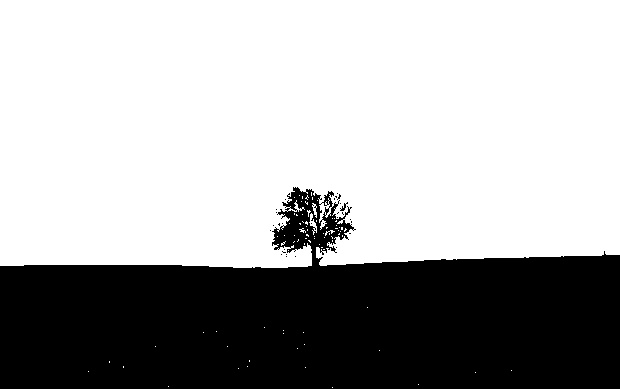
\includegraphics[scale=0.4]{Imagens/resultado_threshold.png}
            \end{figure}
    \end{columns}    
\end{frame}

\subsection{\textit{bits} menos significativos (LSB) e \textit{bits} mais significativos (MSB)}

\begin{frame}{Fundamentação Teórica - LSB e MSB}
    \begin{figure}
        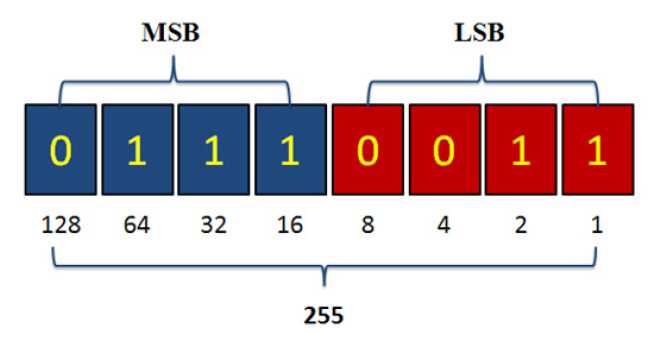
\includegraphics[scale=0.6]{Imagens/lsb_msb_fig.png}
    \end{figure}  
\end{frame}

\subsection{Histograma}

\begin{frame}{Fundamentação Teórica - Histograma}
    \begin{figure}
        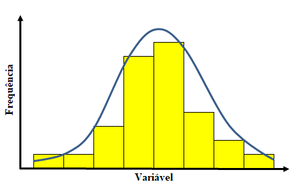
\includegraphics[scale=0.6]{Imagens/histograma_exemplo.png}
    \end{figure}  
\end{frame}

\subsection{Métricas}

\begin{frame}{Fundamentação Teórica - Métricas}
\begin{itemize}
    \item PSNR;
    \item SSIM.
\end{itemize}
    
\end{frame}

\section{Metodologia}

\begin{frame}{Metodologia - Imagens Originais em RGB}
    \begin{figure}
        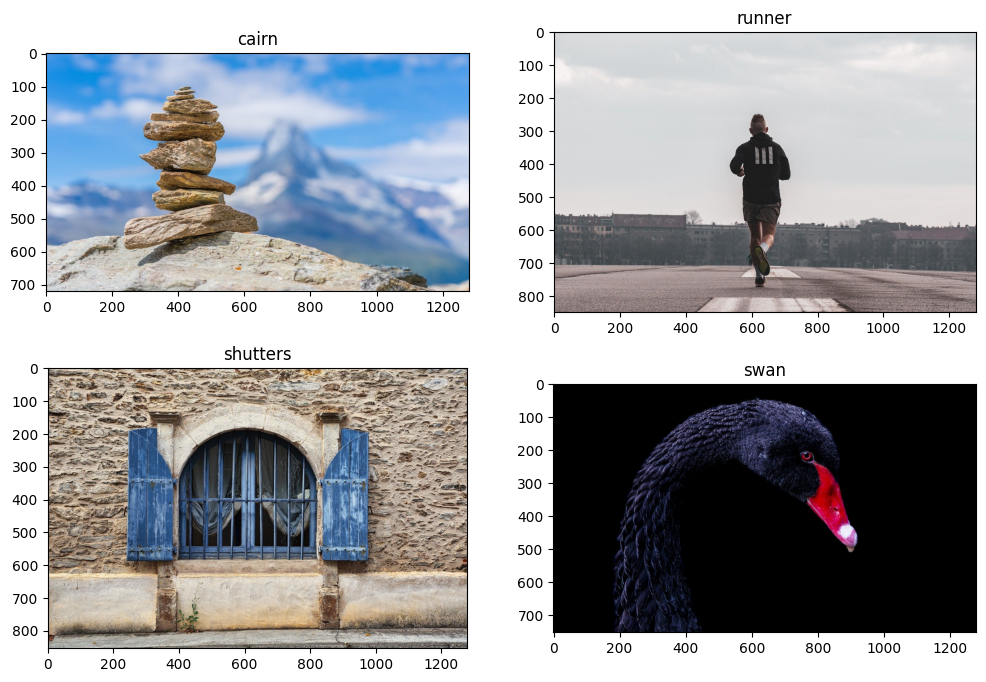
\includegraphics[scale=0.4]{Imagens/metodologia-originais-rgb.png}
    \end{figure}  
\end{frame}

\begin{frame}{Metodologia - Imagens Originais em Tons de Cinza}
    \begin{figure}
        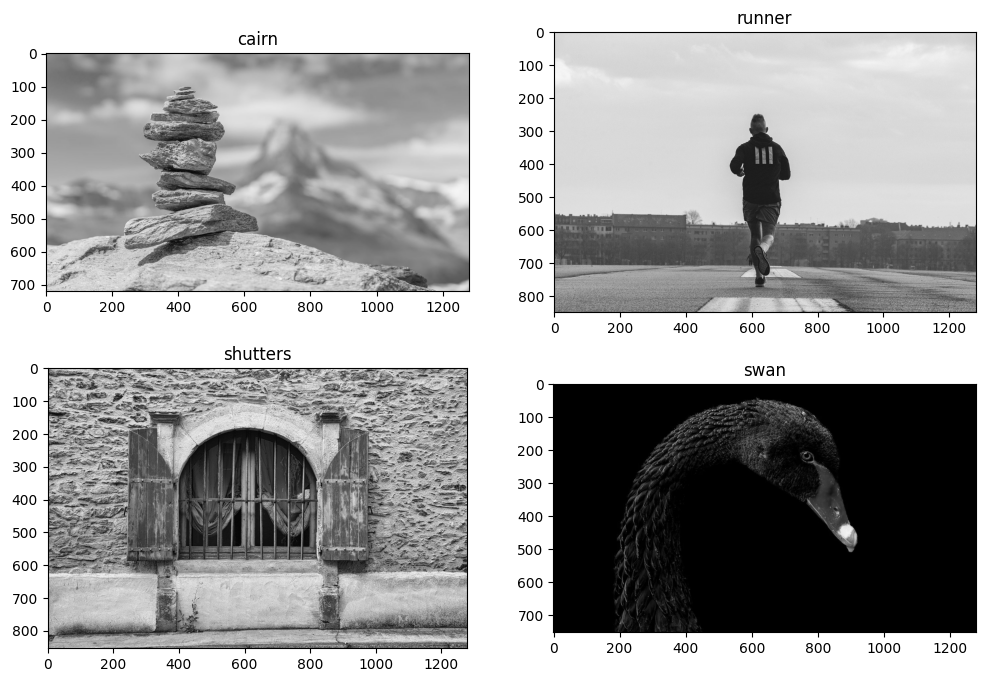
\includegraphics[scale=0.4]{Imagens/imagens-originais-gray.png}
    \end{figure}  
\end{frame}

\begin{frame}{Metodologia - Informação Espacial}
    \begin{figure}
        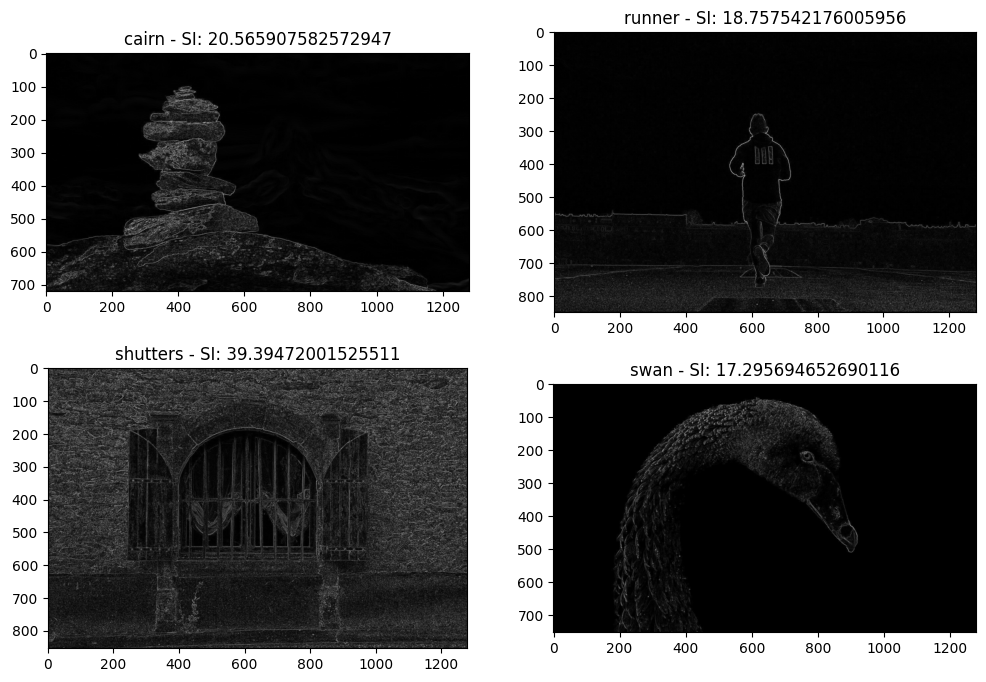
\includegraphics[scale=0.4]{Imagens/metodologia-si.png}
    \end{figure}  
\end{frame}

\begin{frame}{Metodologia - Ambiente Google Colab/Python}
    \begin{figure}
        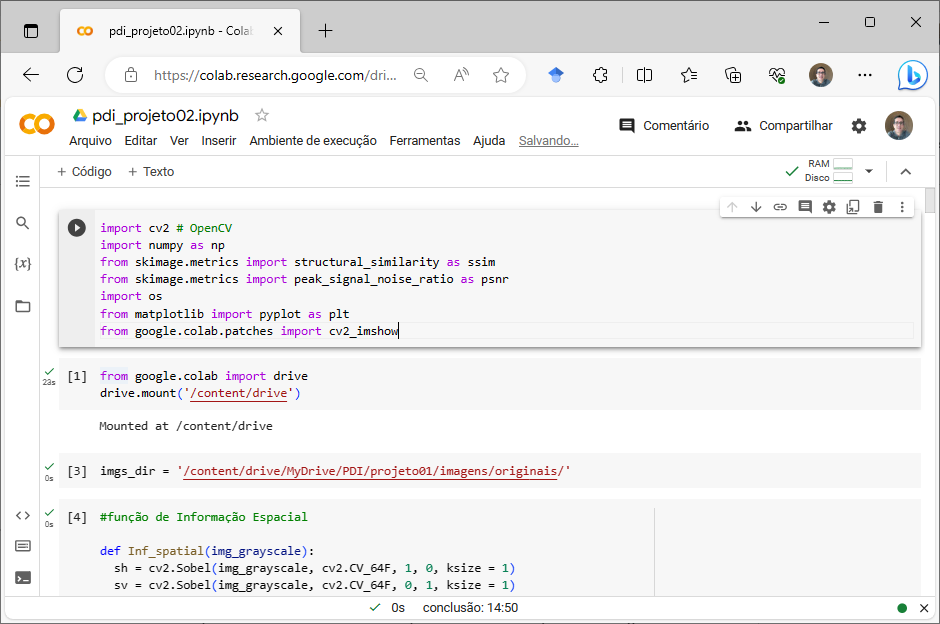
\includegraphics[scale=0.4]{Imagens/metodologia-colab.png}
    \end{figure}  
\end{frame}

\section{Resultados}

\begin{frame}{Resultados - Histograma das Imagens Originais}
\begin{figure}
    \begin{tabular}{cc}
         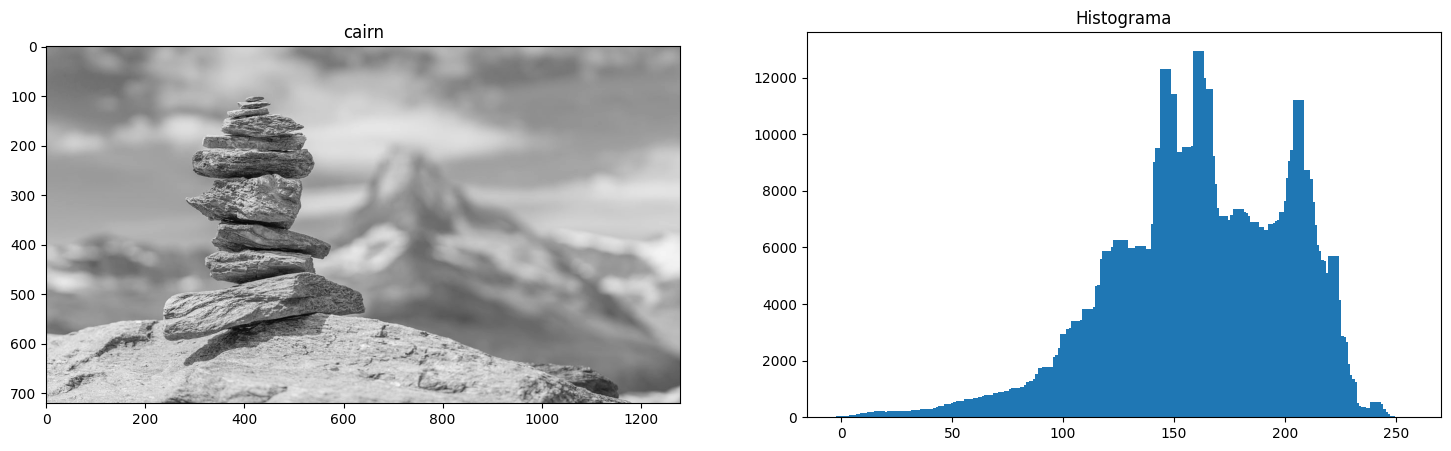
\includegraphics[scale=0.15]{Imagens/resultados-histograma-cairn.png} &   
         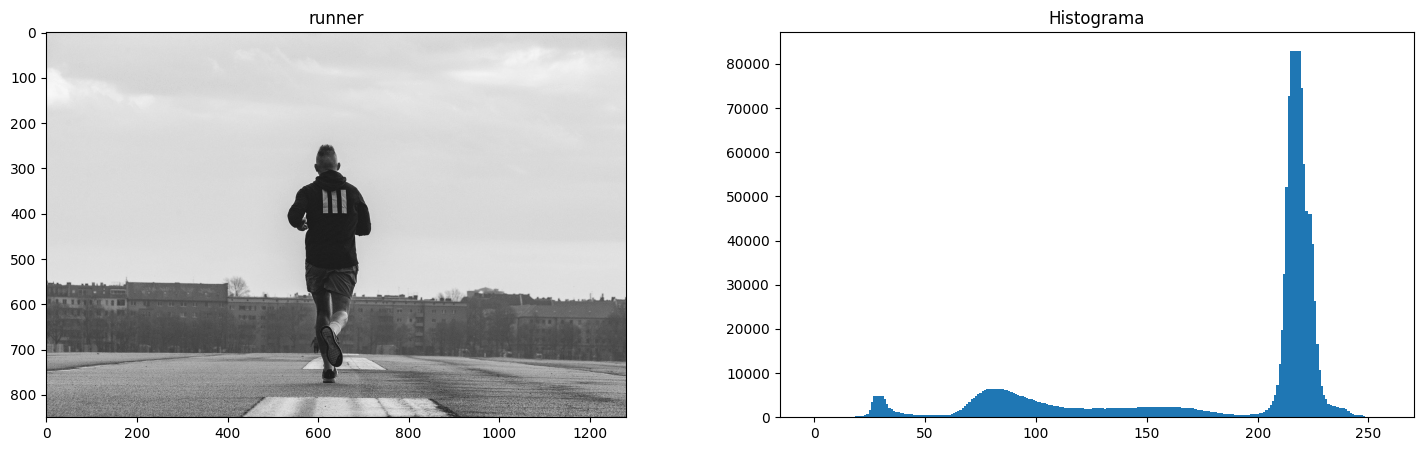
\includegraphics[scale=0.15]{Imagens/resultados-histograma-runner.png} \\
         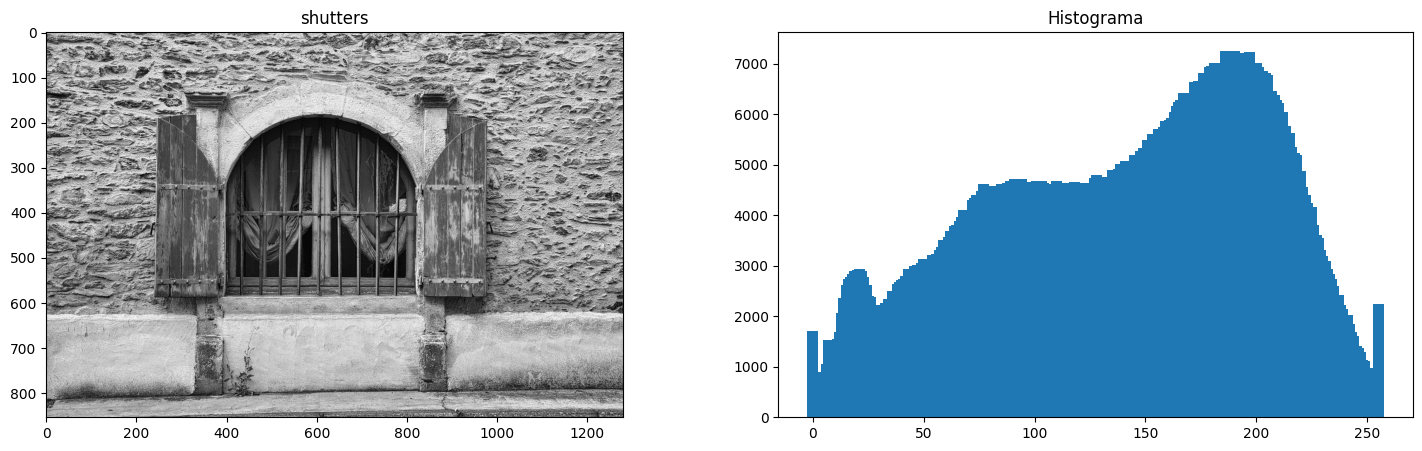
\includegraphics[scale=0.15]{Imagens/resultados-histograma-shutters.png} &   
         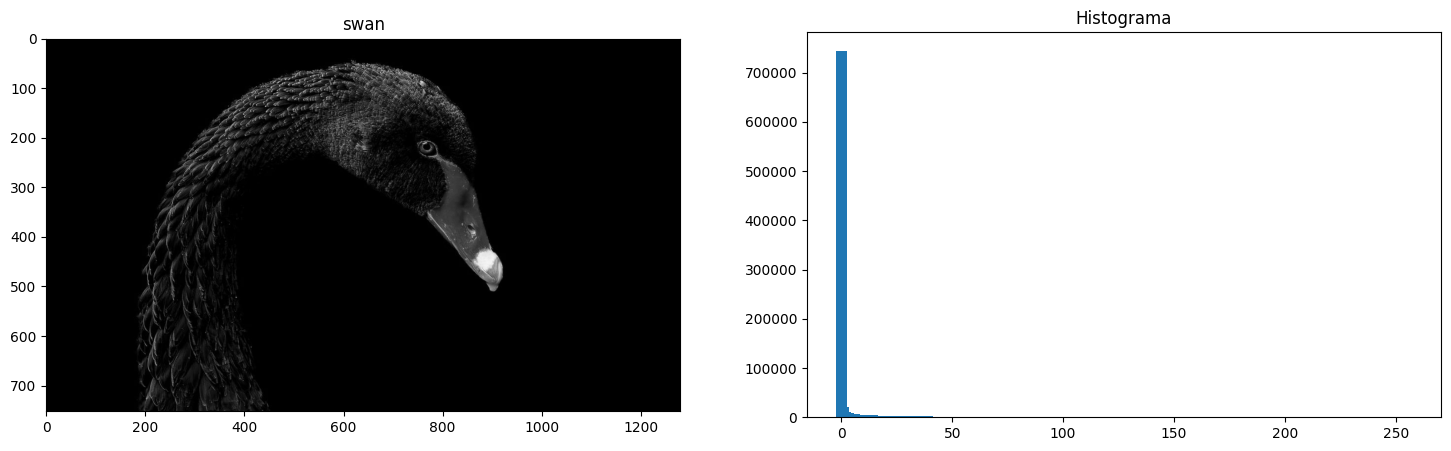
\includegraphics[scale=0.15]{Imagens/resultados-histograma-swan.png} \\
    \end{tabular}
\end{figure}
\end{frame}

\begin{frame}{Resultados - Transformação de Intensidade}
    \begin{figure}
        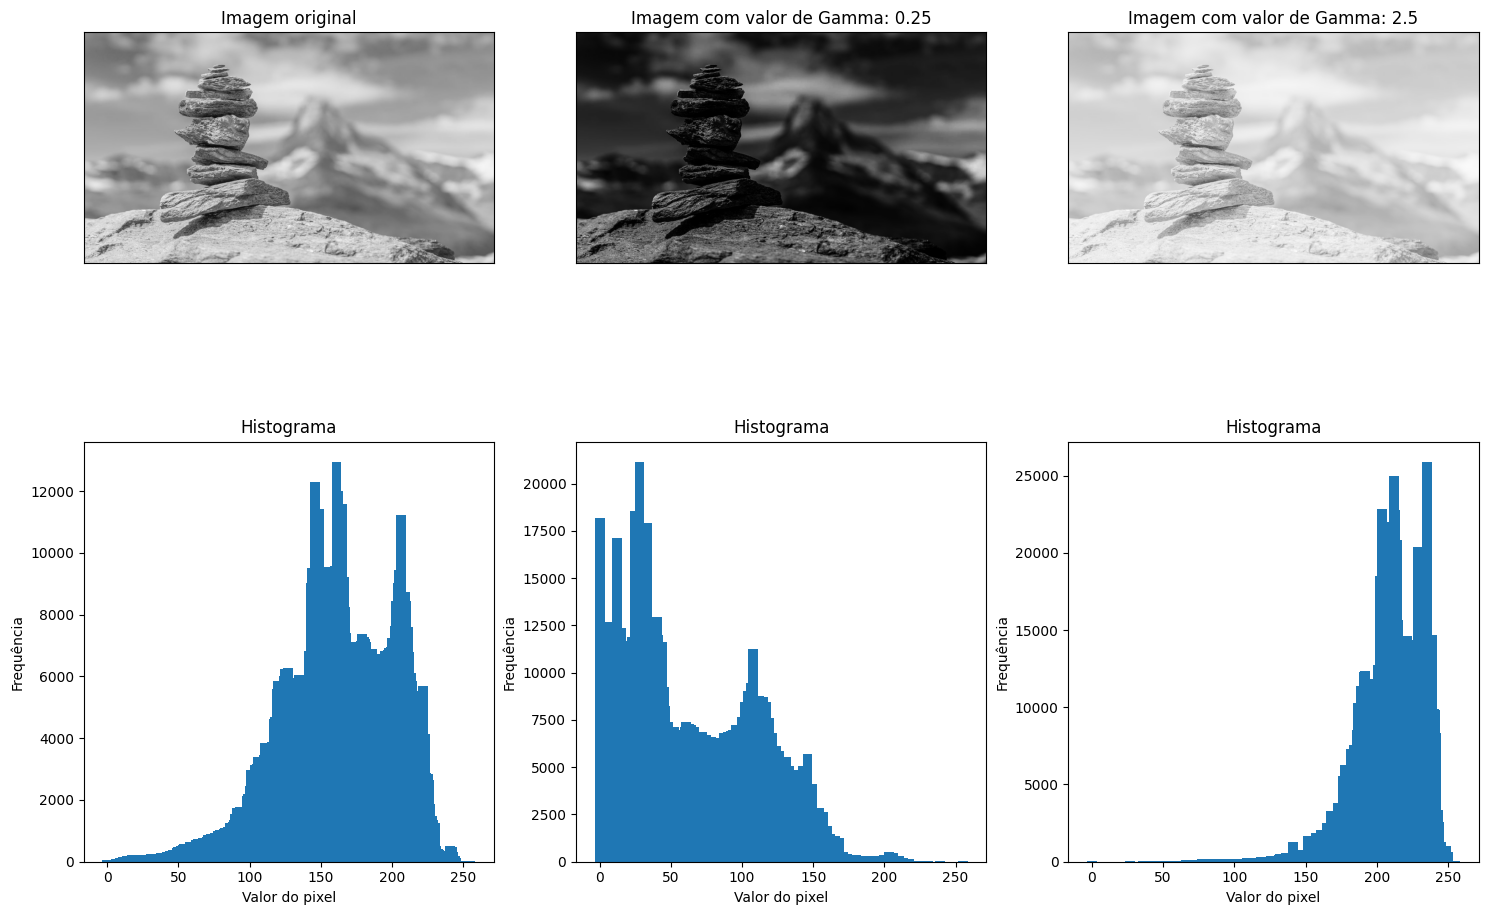
\includegraphics[scale=0.25]{Imagens/resultados-gamma-cairn.png}
    \end{figure}  
\end{frame}

\begin{frame}{Resultados - Transformação de Intensidade}
    \begin{figure}
        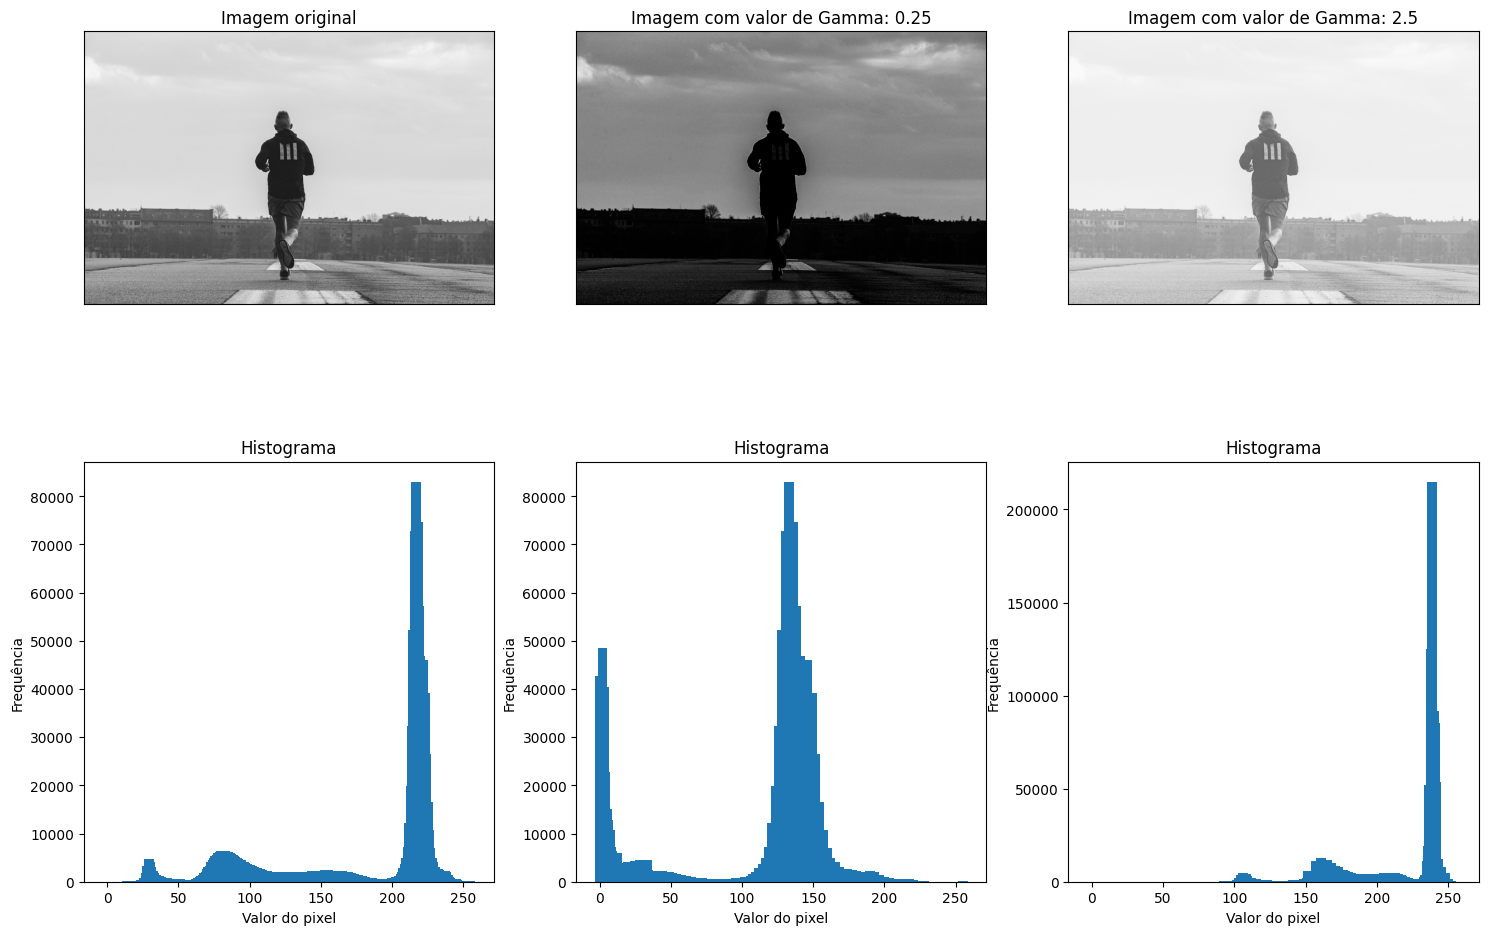
\includegraphics[scale=0.25]{Imagens/resultados-gamma-runner.png}
    \end{figure}  
\end{frame}

\begin{frame}{Resultados - Transformação de Intensidade}
    \begin{figure}
        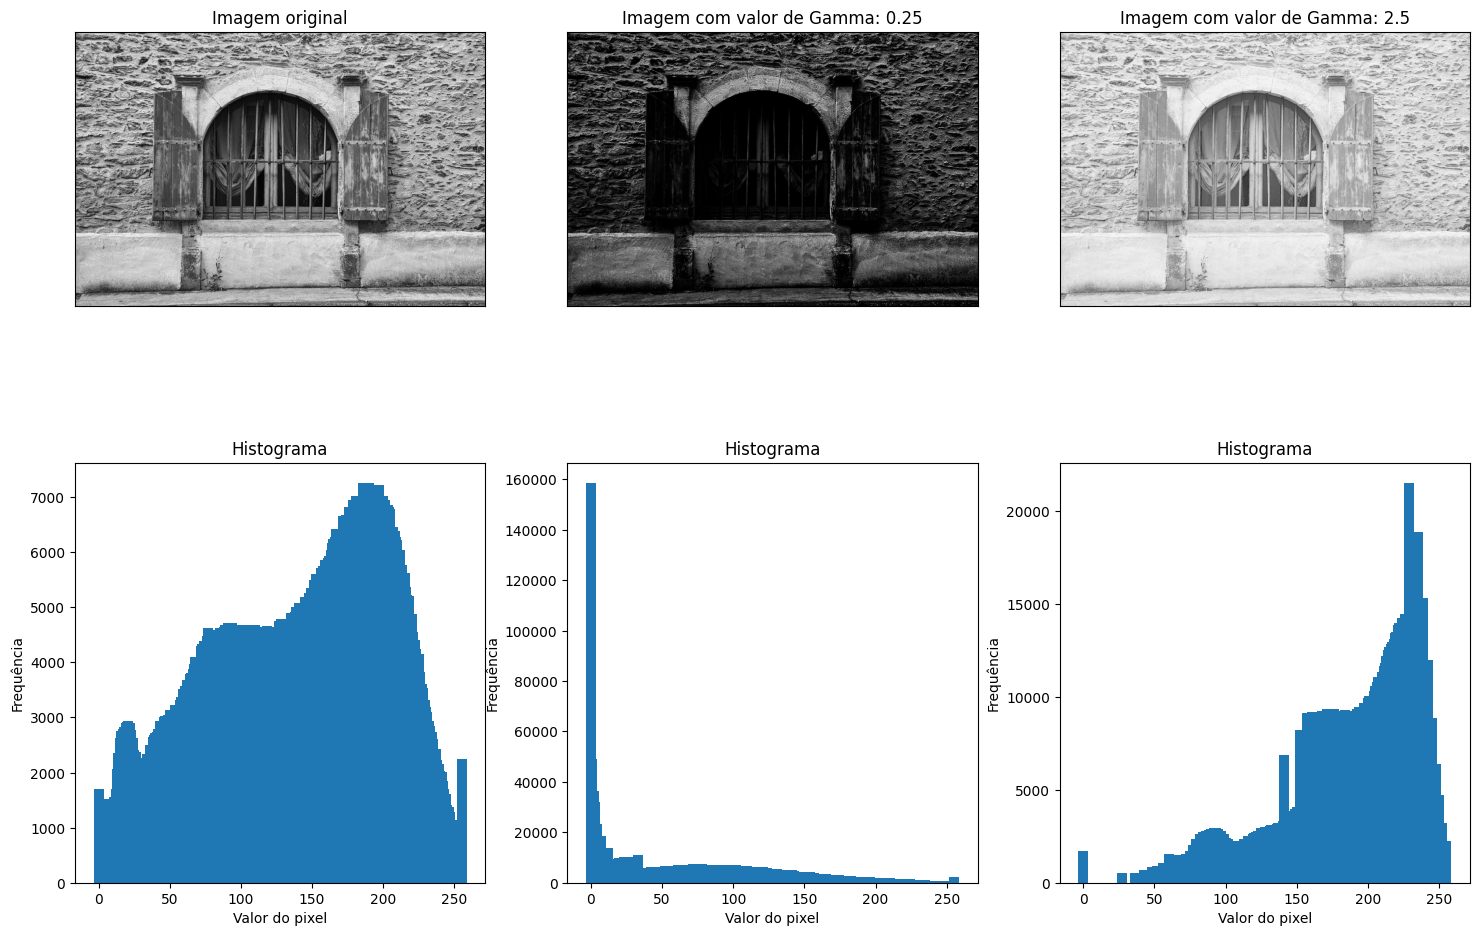
\includegraphics[scale=0.25]{Imagens/resultados-gamma-shutters.png}
    \end{figure}  
\end{frame}

\begin{frame}{Resultados - Transformação de Intensidade}
    \begin{figure}
        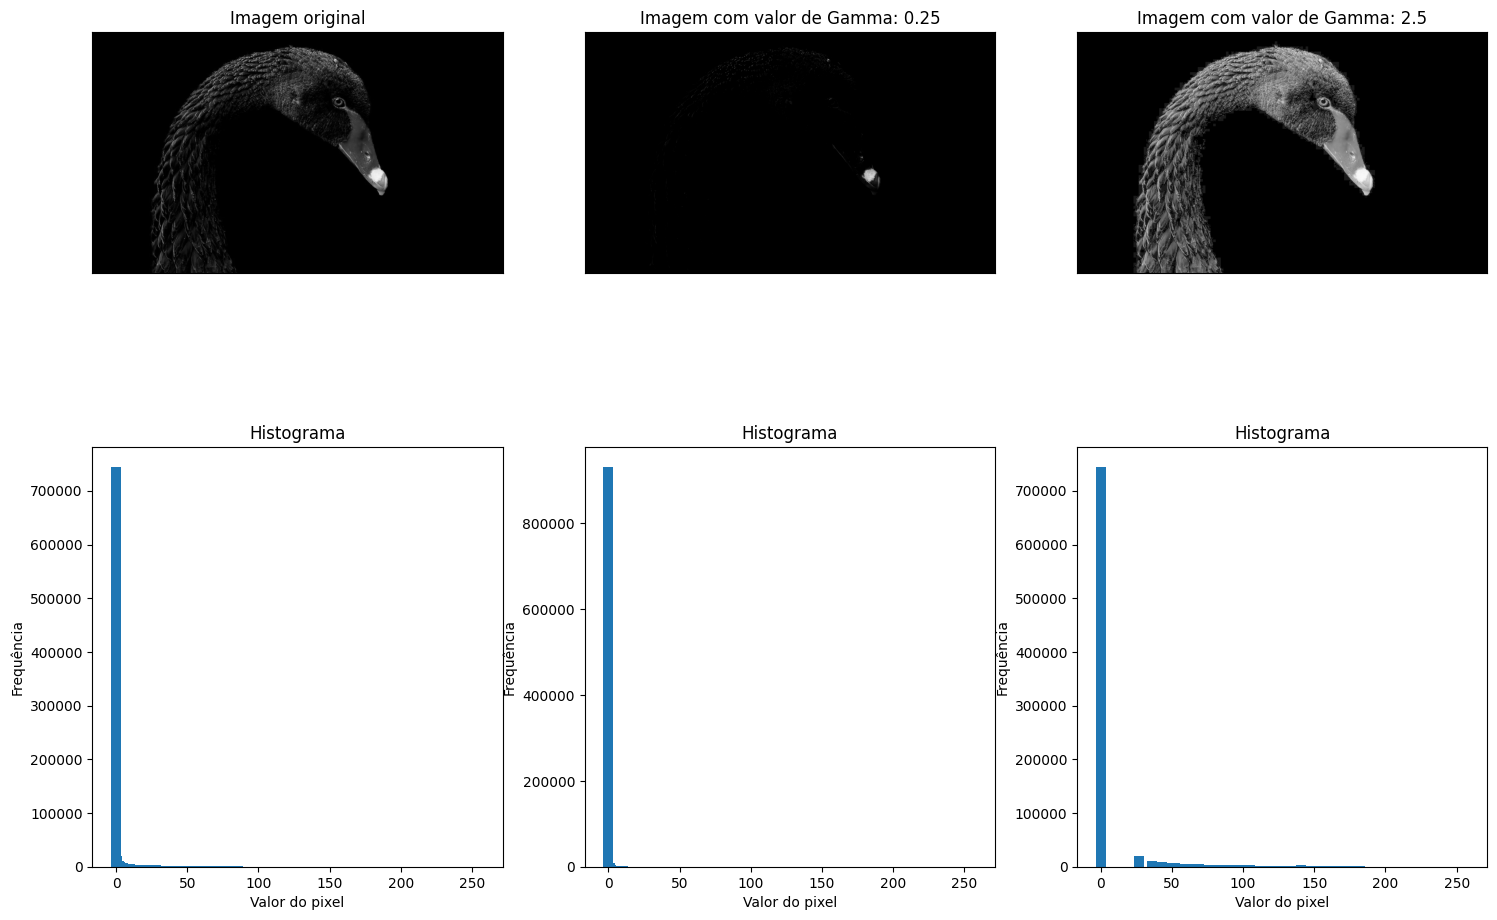
\includegraphics[scale=0.25]{Imagens/resultados-gamma-swam.png}
    \end{figure}  
\end{frame}

\begin{frame}{Resultados - Binarização}
    \begin{figure}
        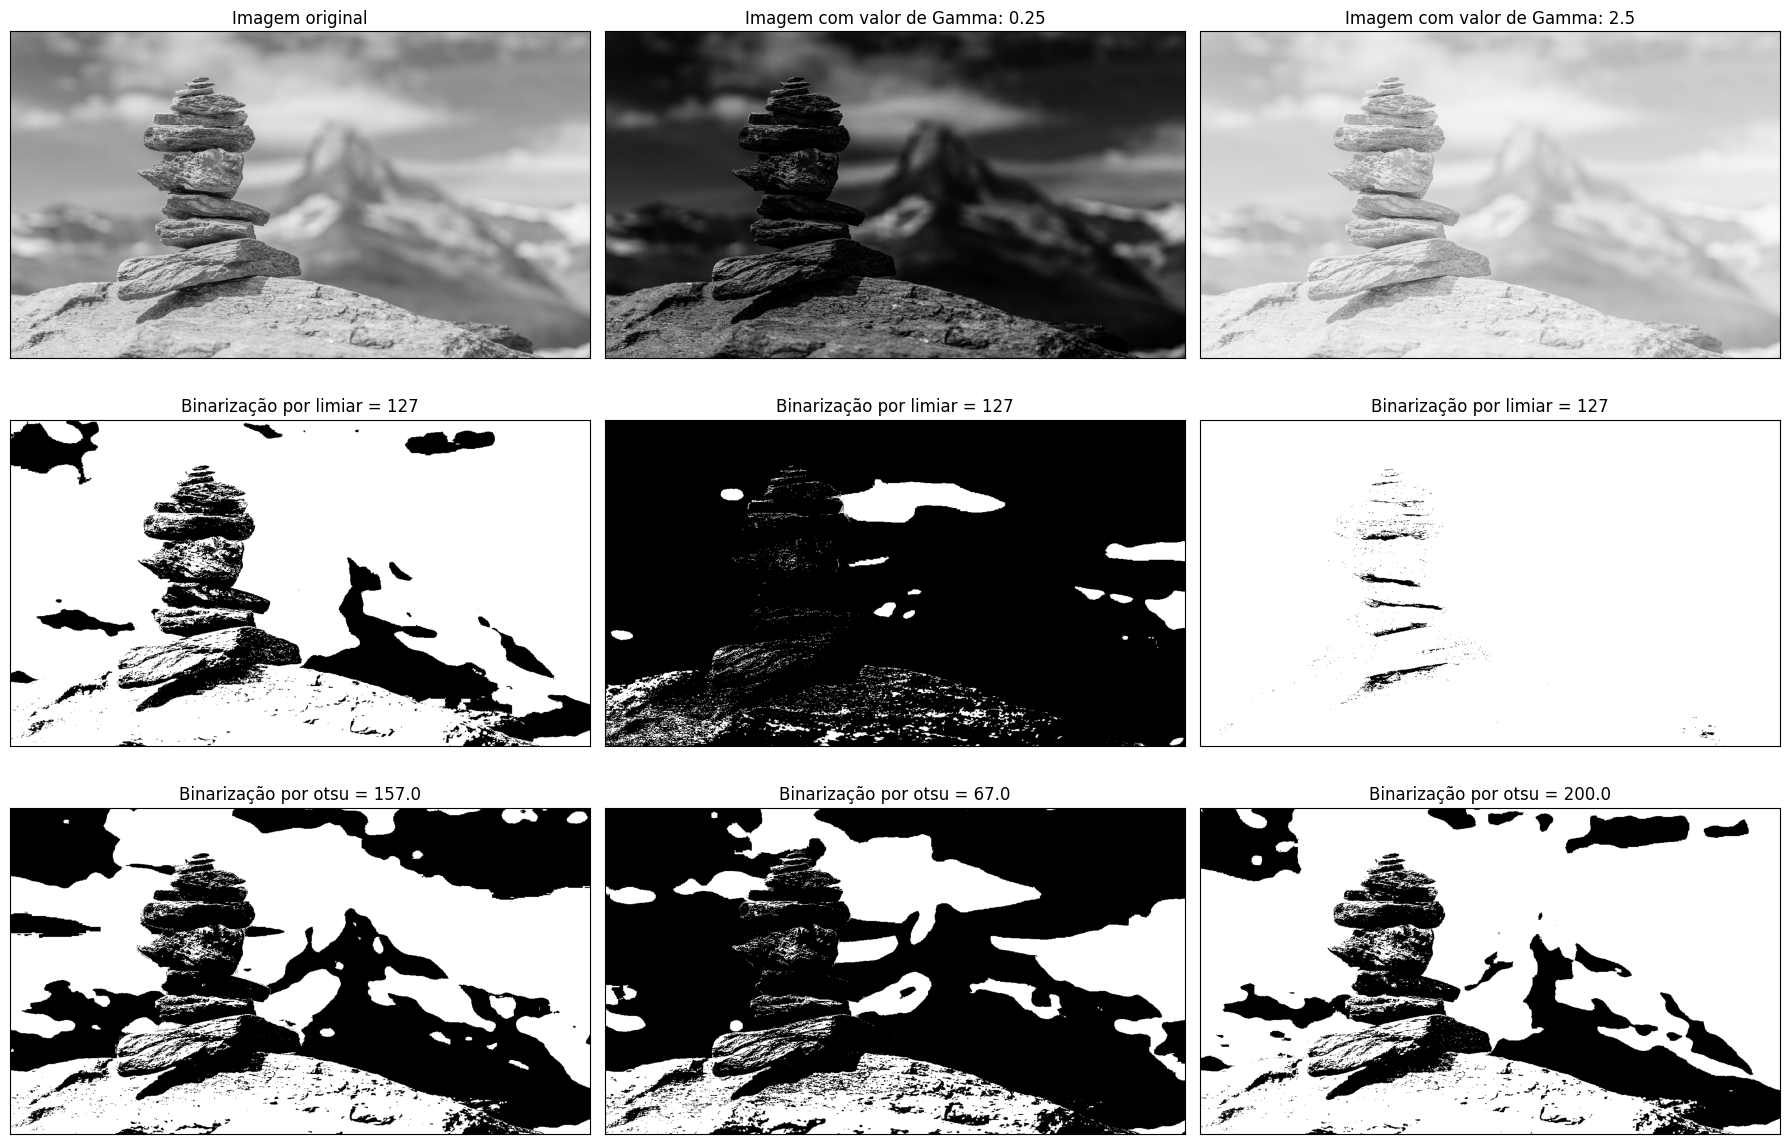
\includegraphics[scale=0.23]{Imagens/resultados-binarizacao-cairn.png}
    \end{figure}  
\end{frame}

\begin{frame}{Resultados - Binarização}
    \begin{figure}
        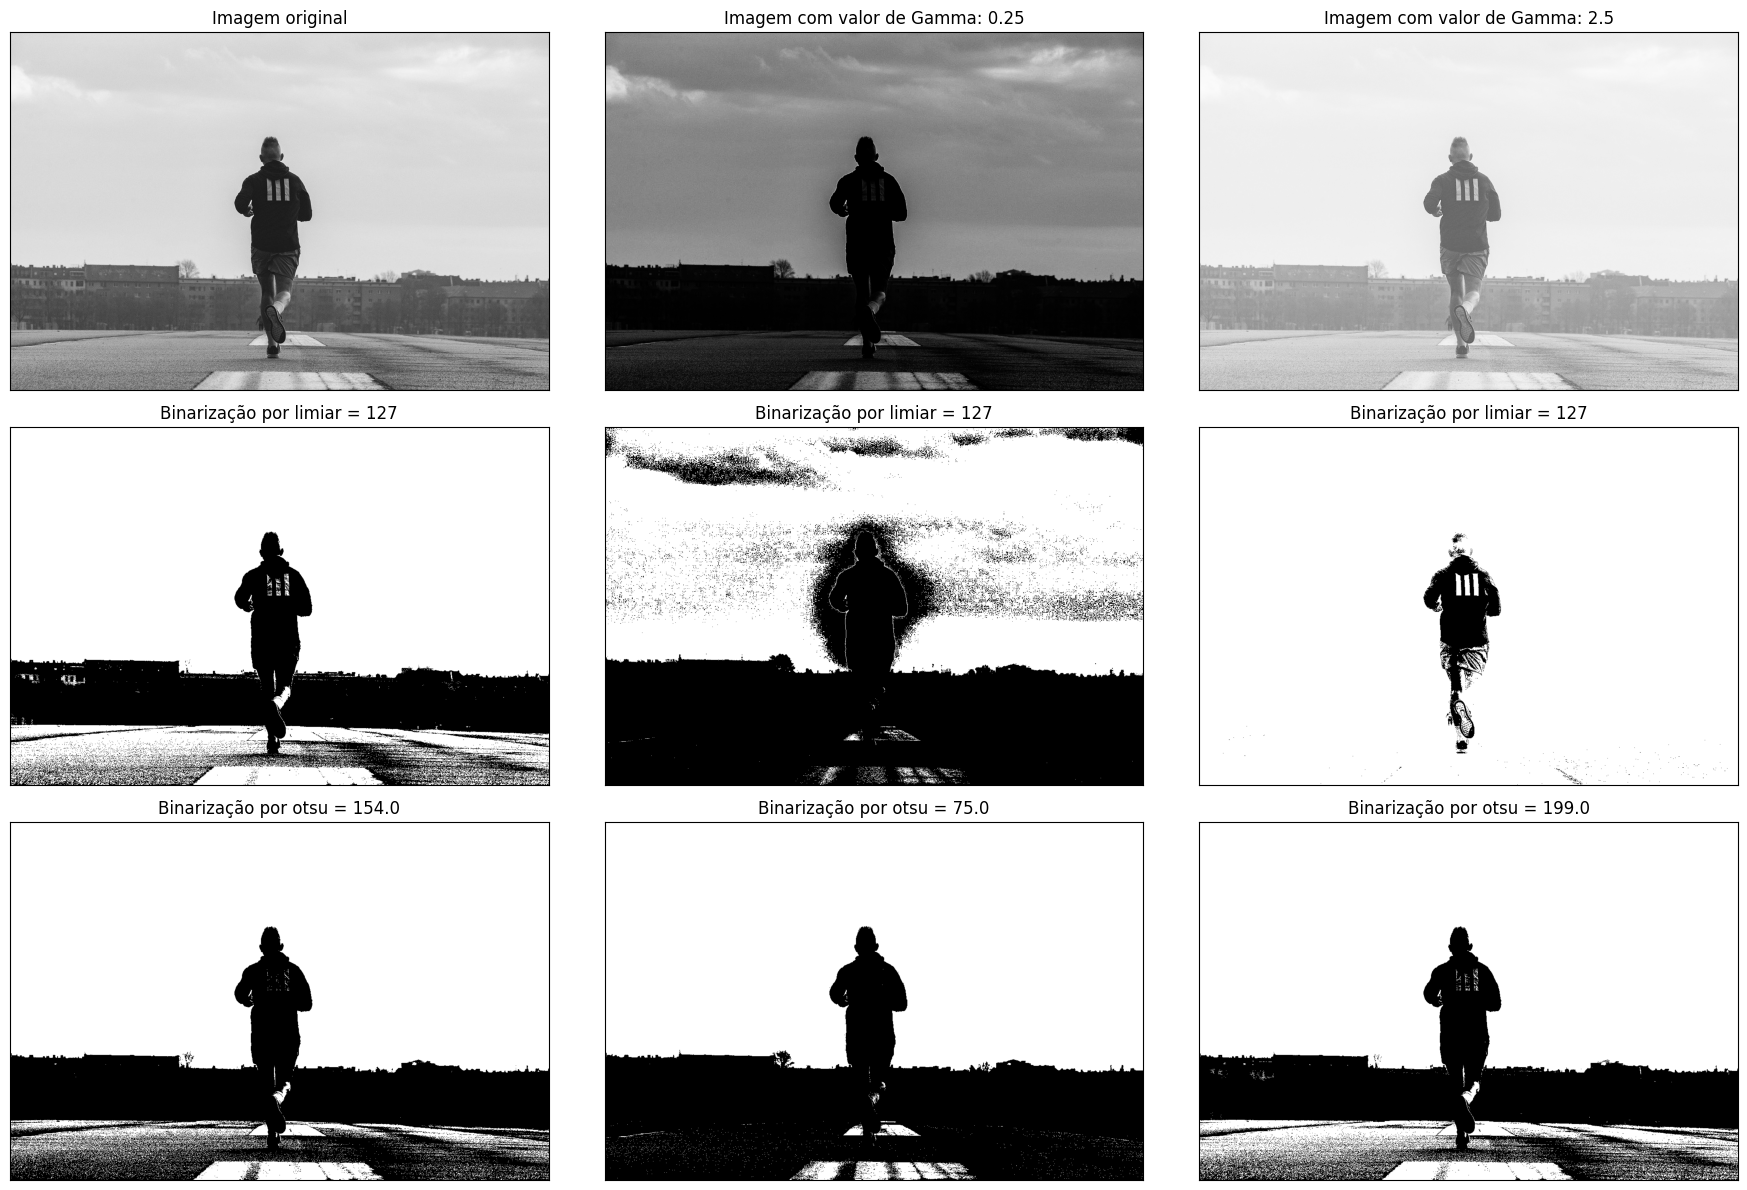
\includegraphics[scale=0.23]{Imagens/resultados-binarizacao-runner.png}
    \end{figure}  
\end{frame}

\begin{frame}{Resultados - Binarização}
    \begin{figure}
        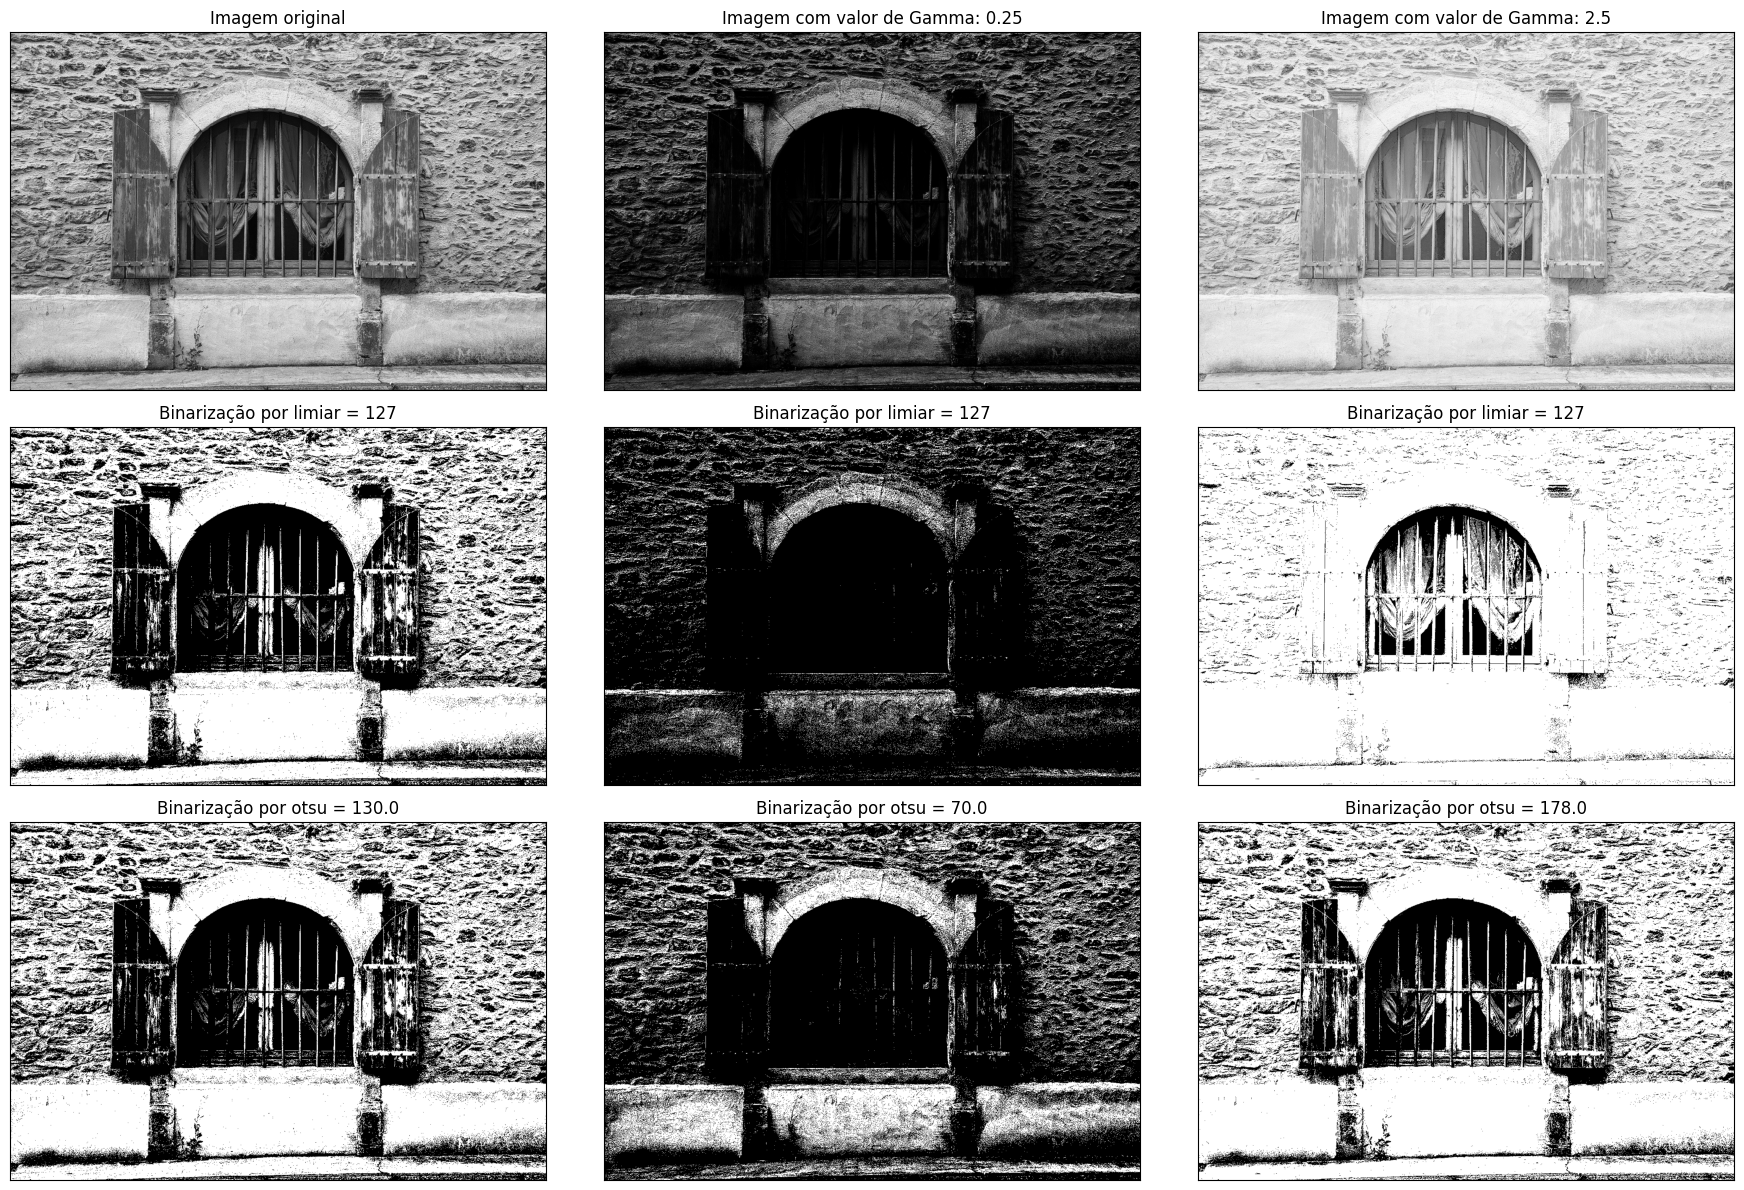
\includegraphics[scale=0.23]{Imagens/resultados-binarizacao-shutters.png}
    \end{figure}  
\end{frame}

\begin{frame}{Resultados - Binarização}
    \begin{figure}
        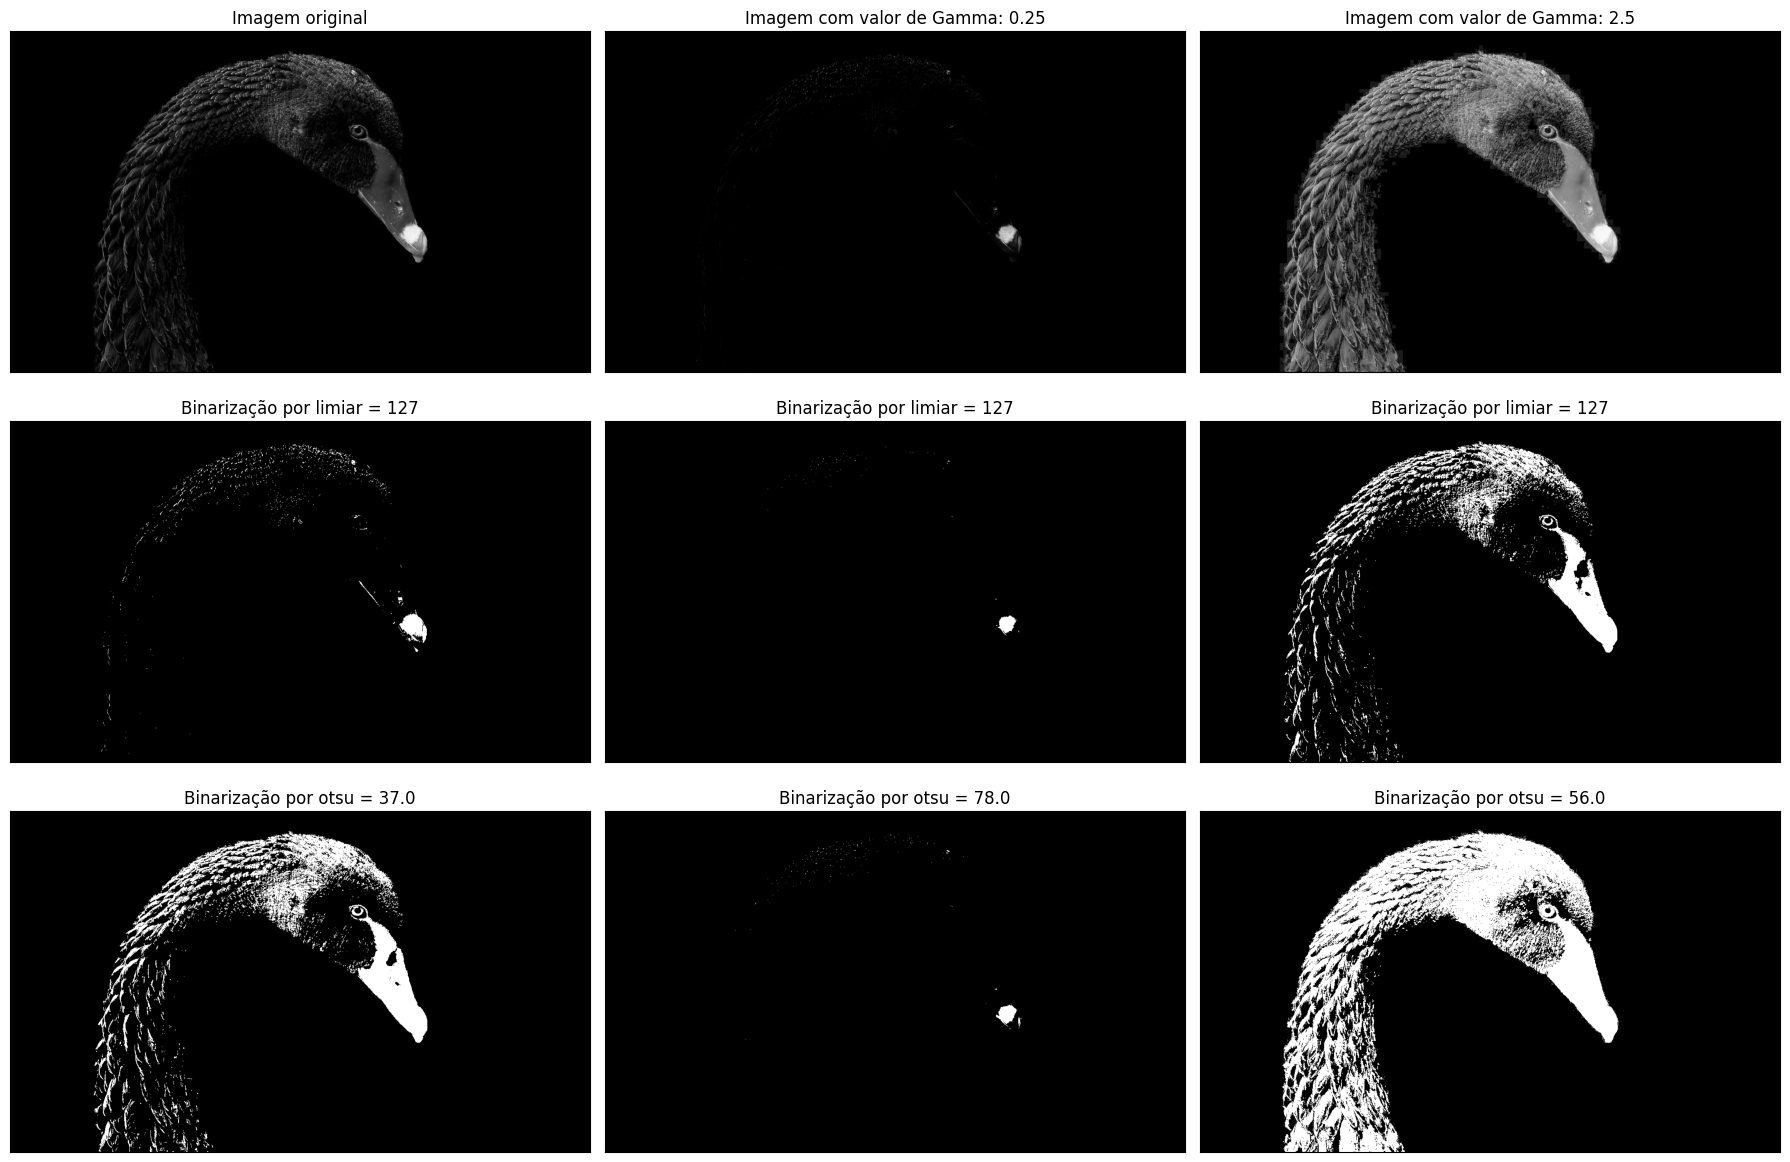
\includegraphics[scale=0.23]{Imagens/resultados-binarizacao-swan.png}
    \end{figure}  
\end{frame}

\begin{frame}{Resultados - LSB}
    \begin{figure}
        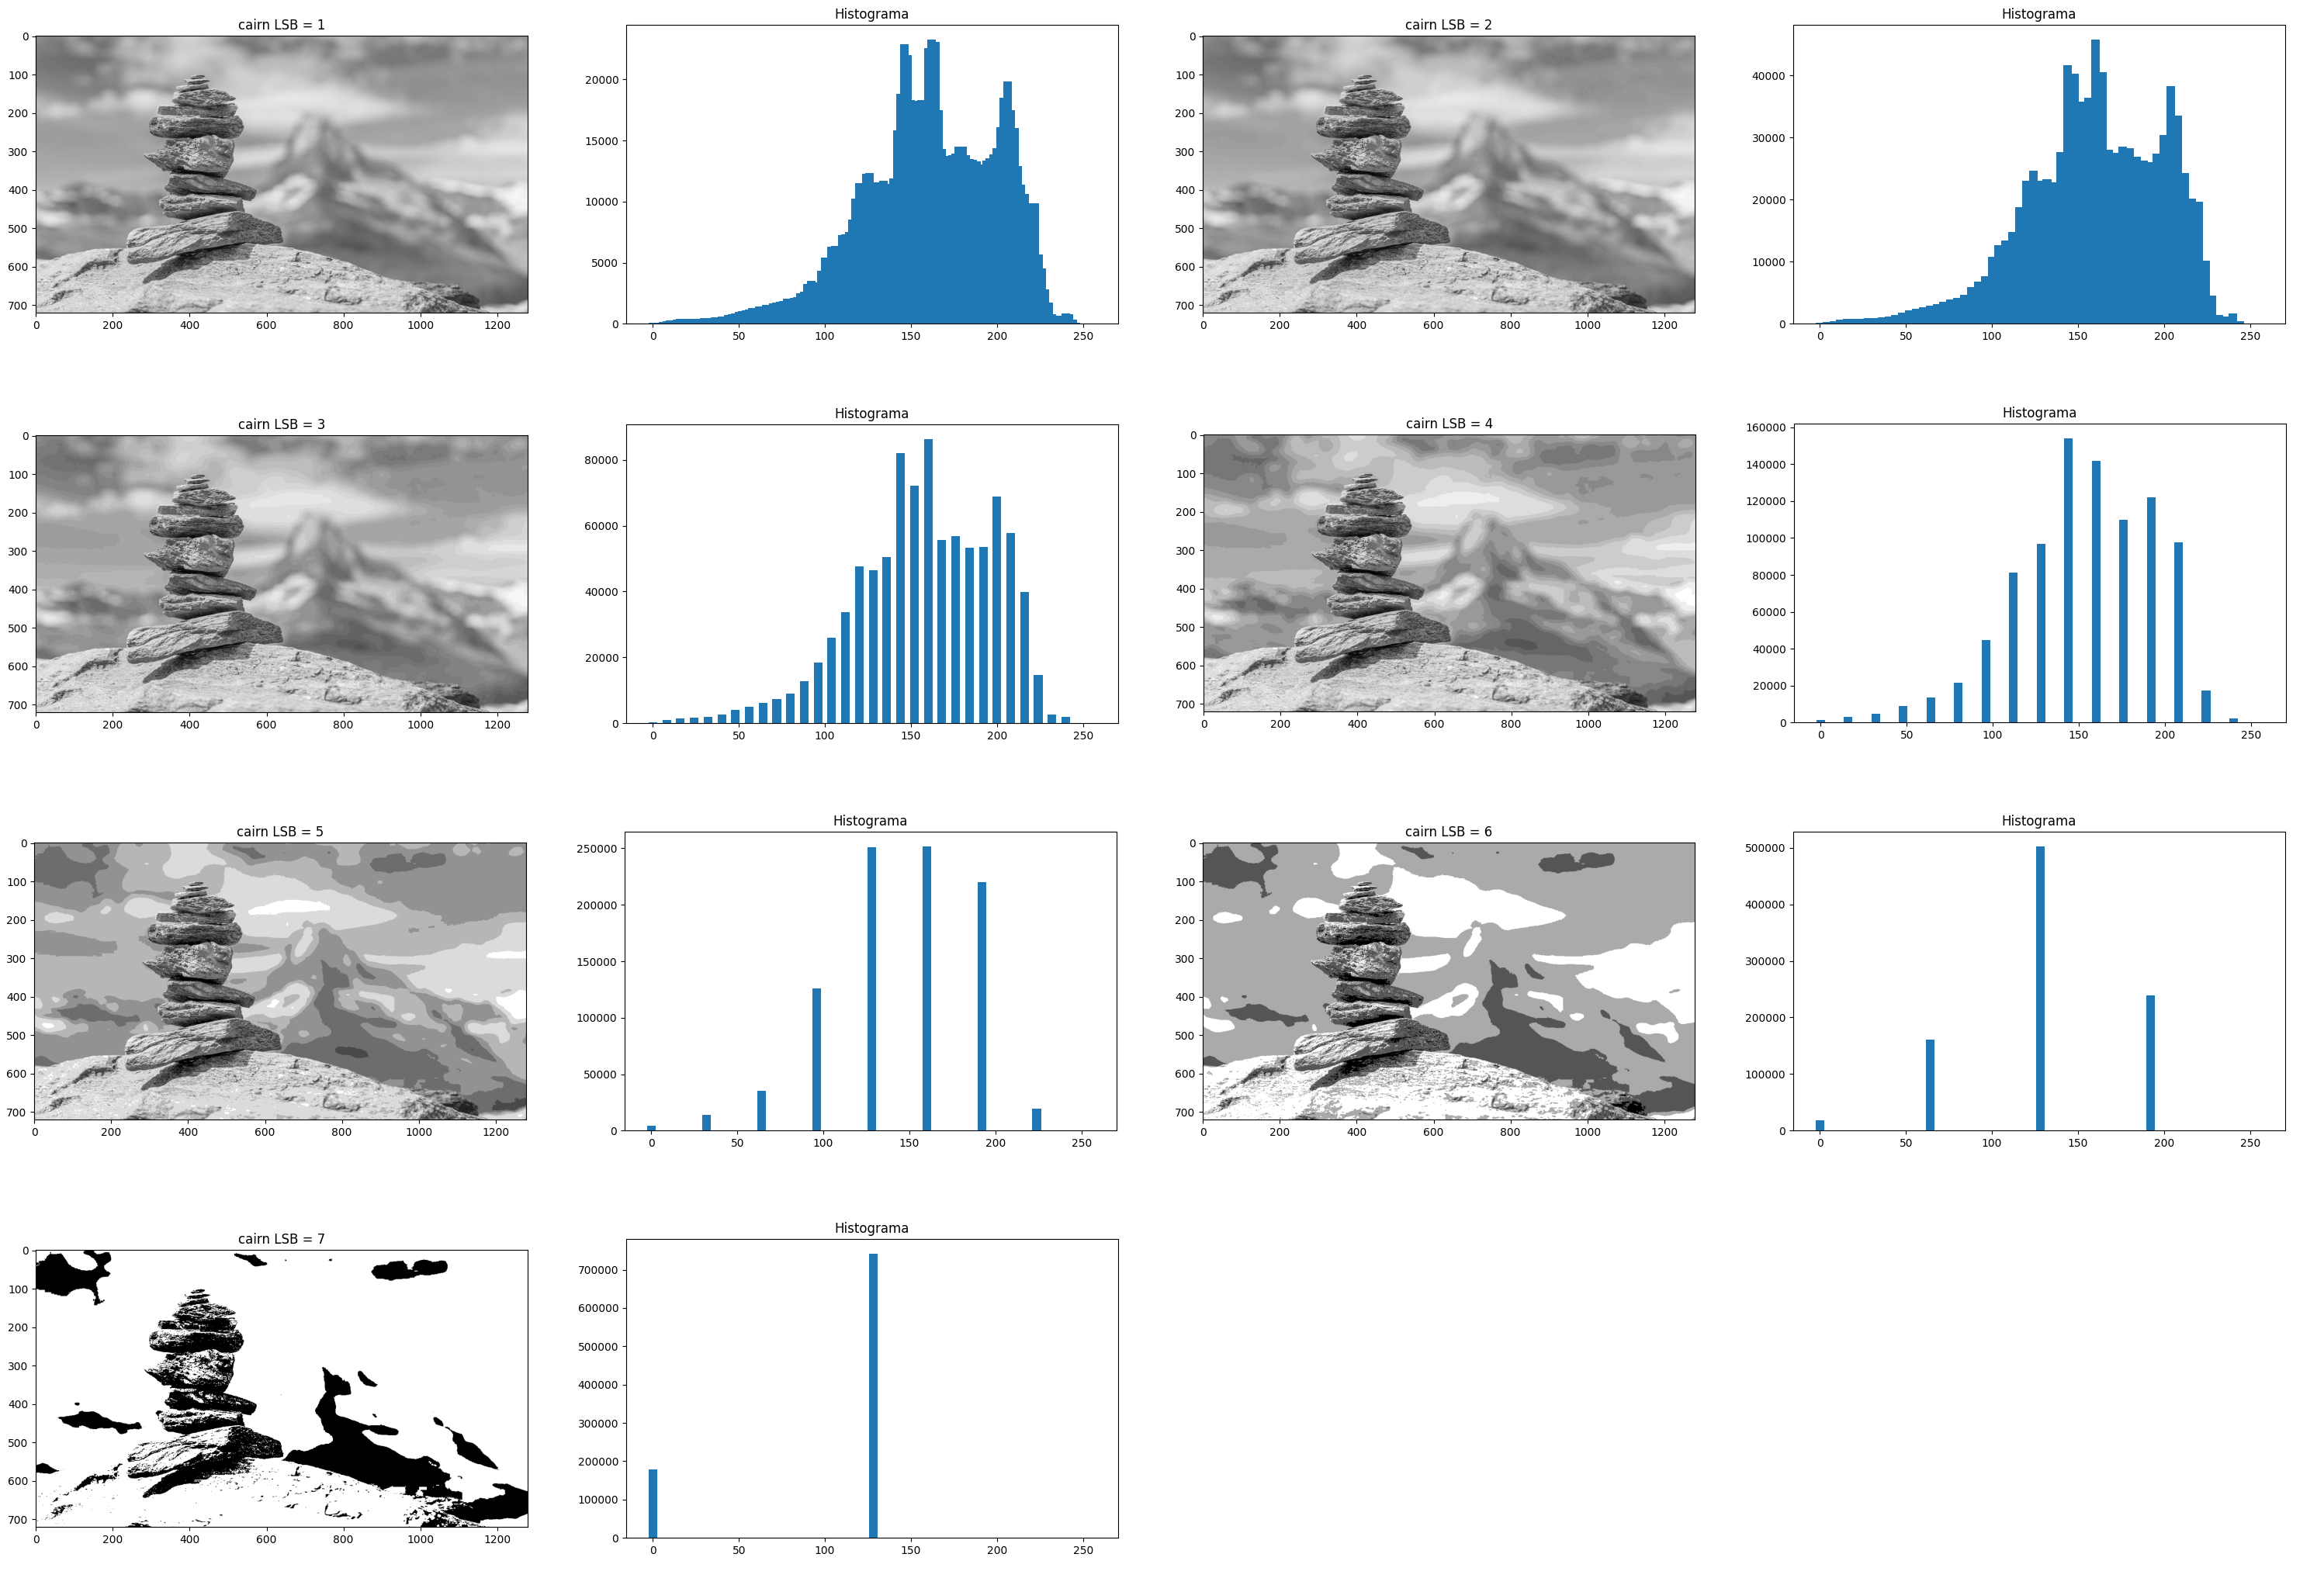
\includegraphics[scale=0.16]{Imagens/resultados-cairn-lsb.png}
    \end{figure}  
\end{frame}

\begin{frame}{Resultados - LSB}
    \begin{figure}
        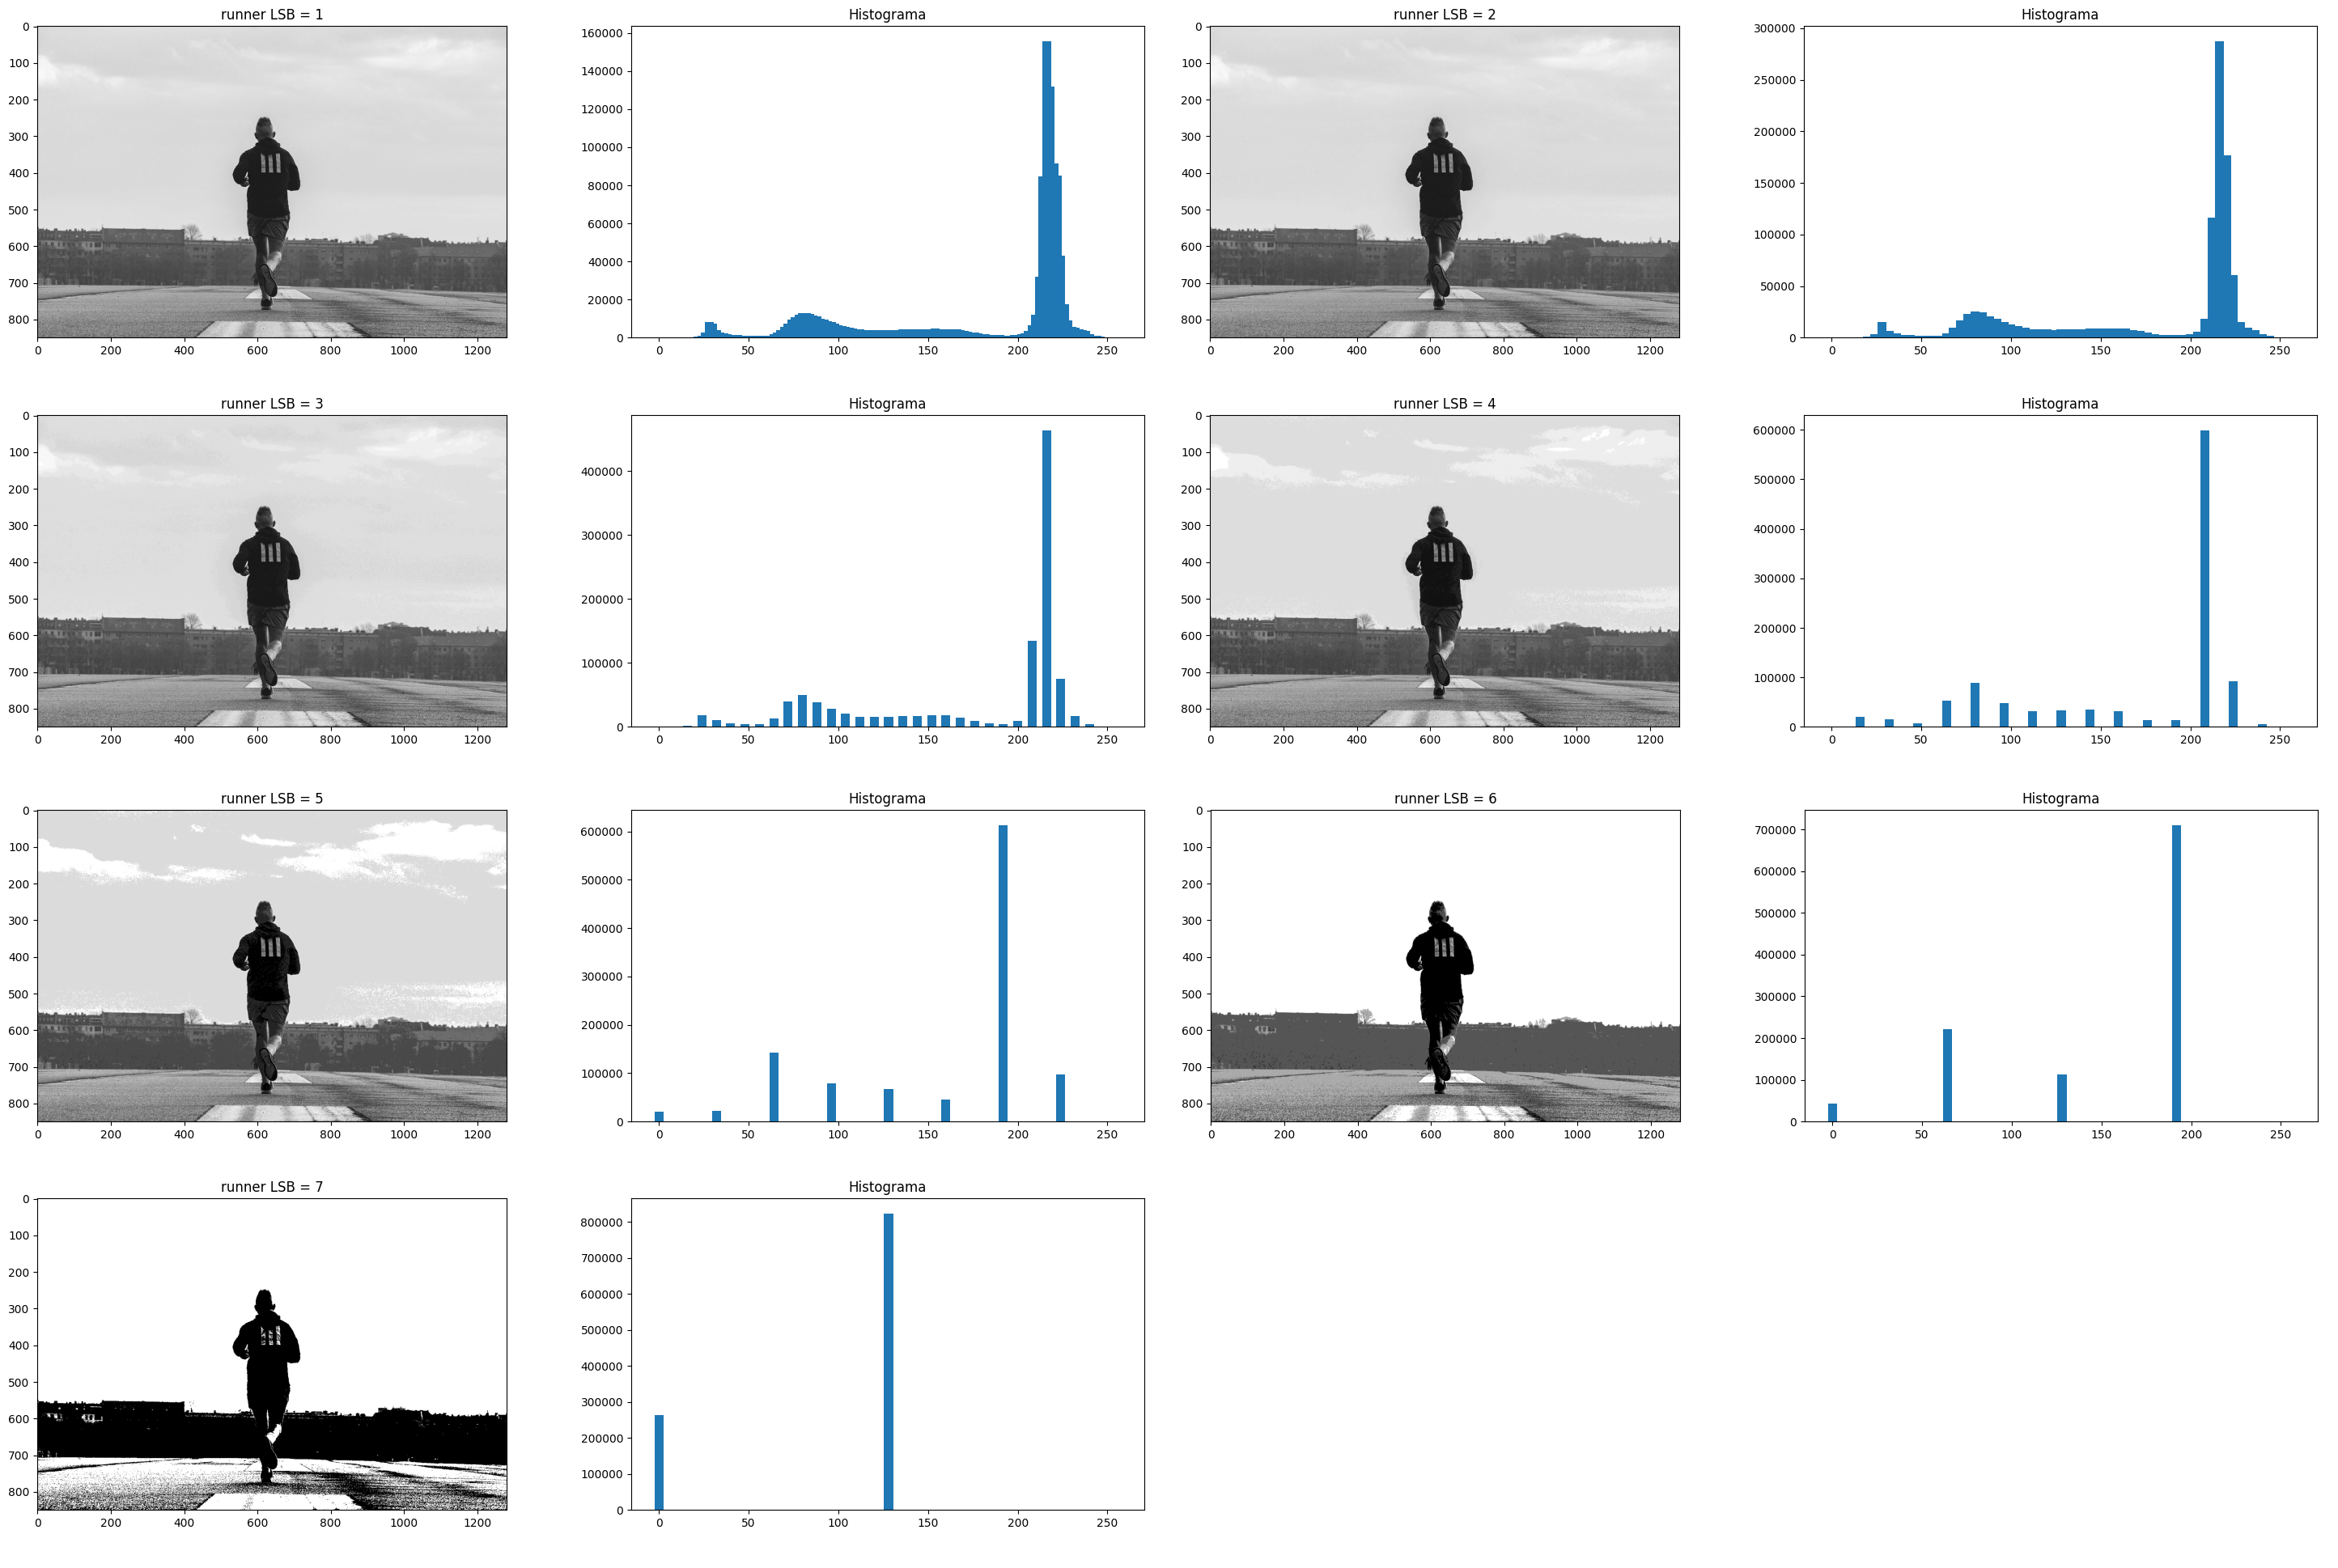
\includegraphics[scale=0.16]{Imagens/resultados-runner-lsb.png}
    \end{figure}  
\end{frame}

\begin{frame}{Resultados - LSB}
    \begin{figure}
        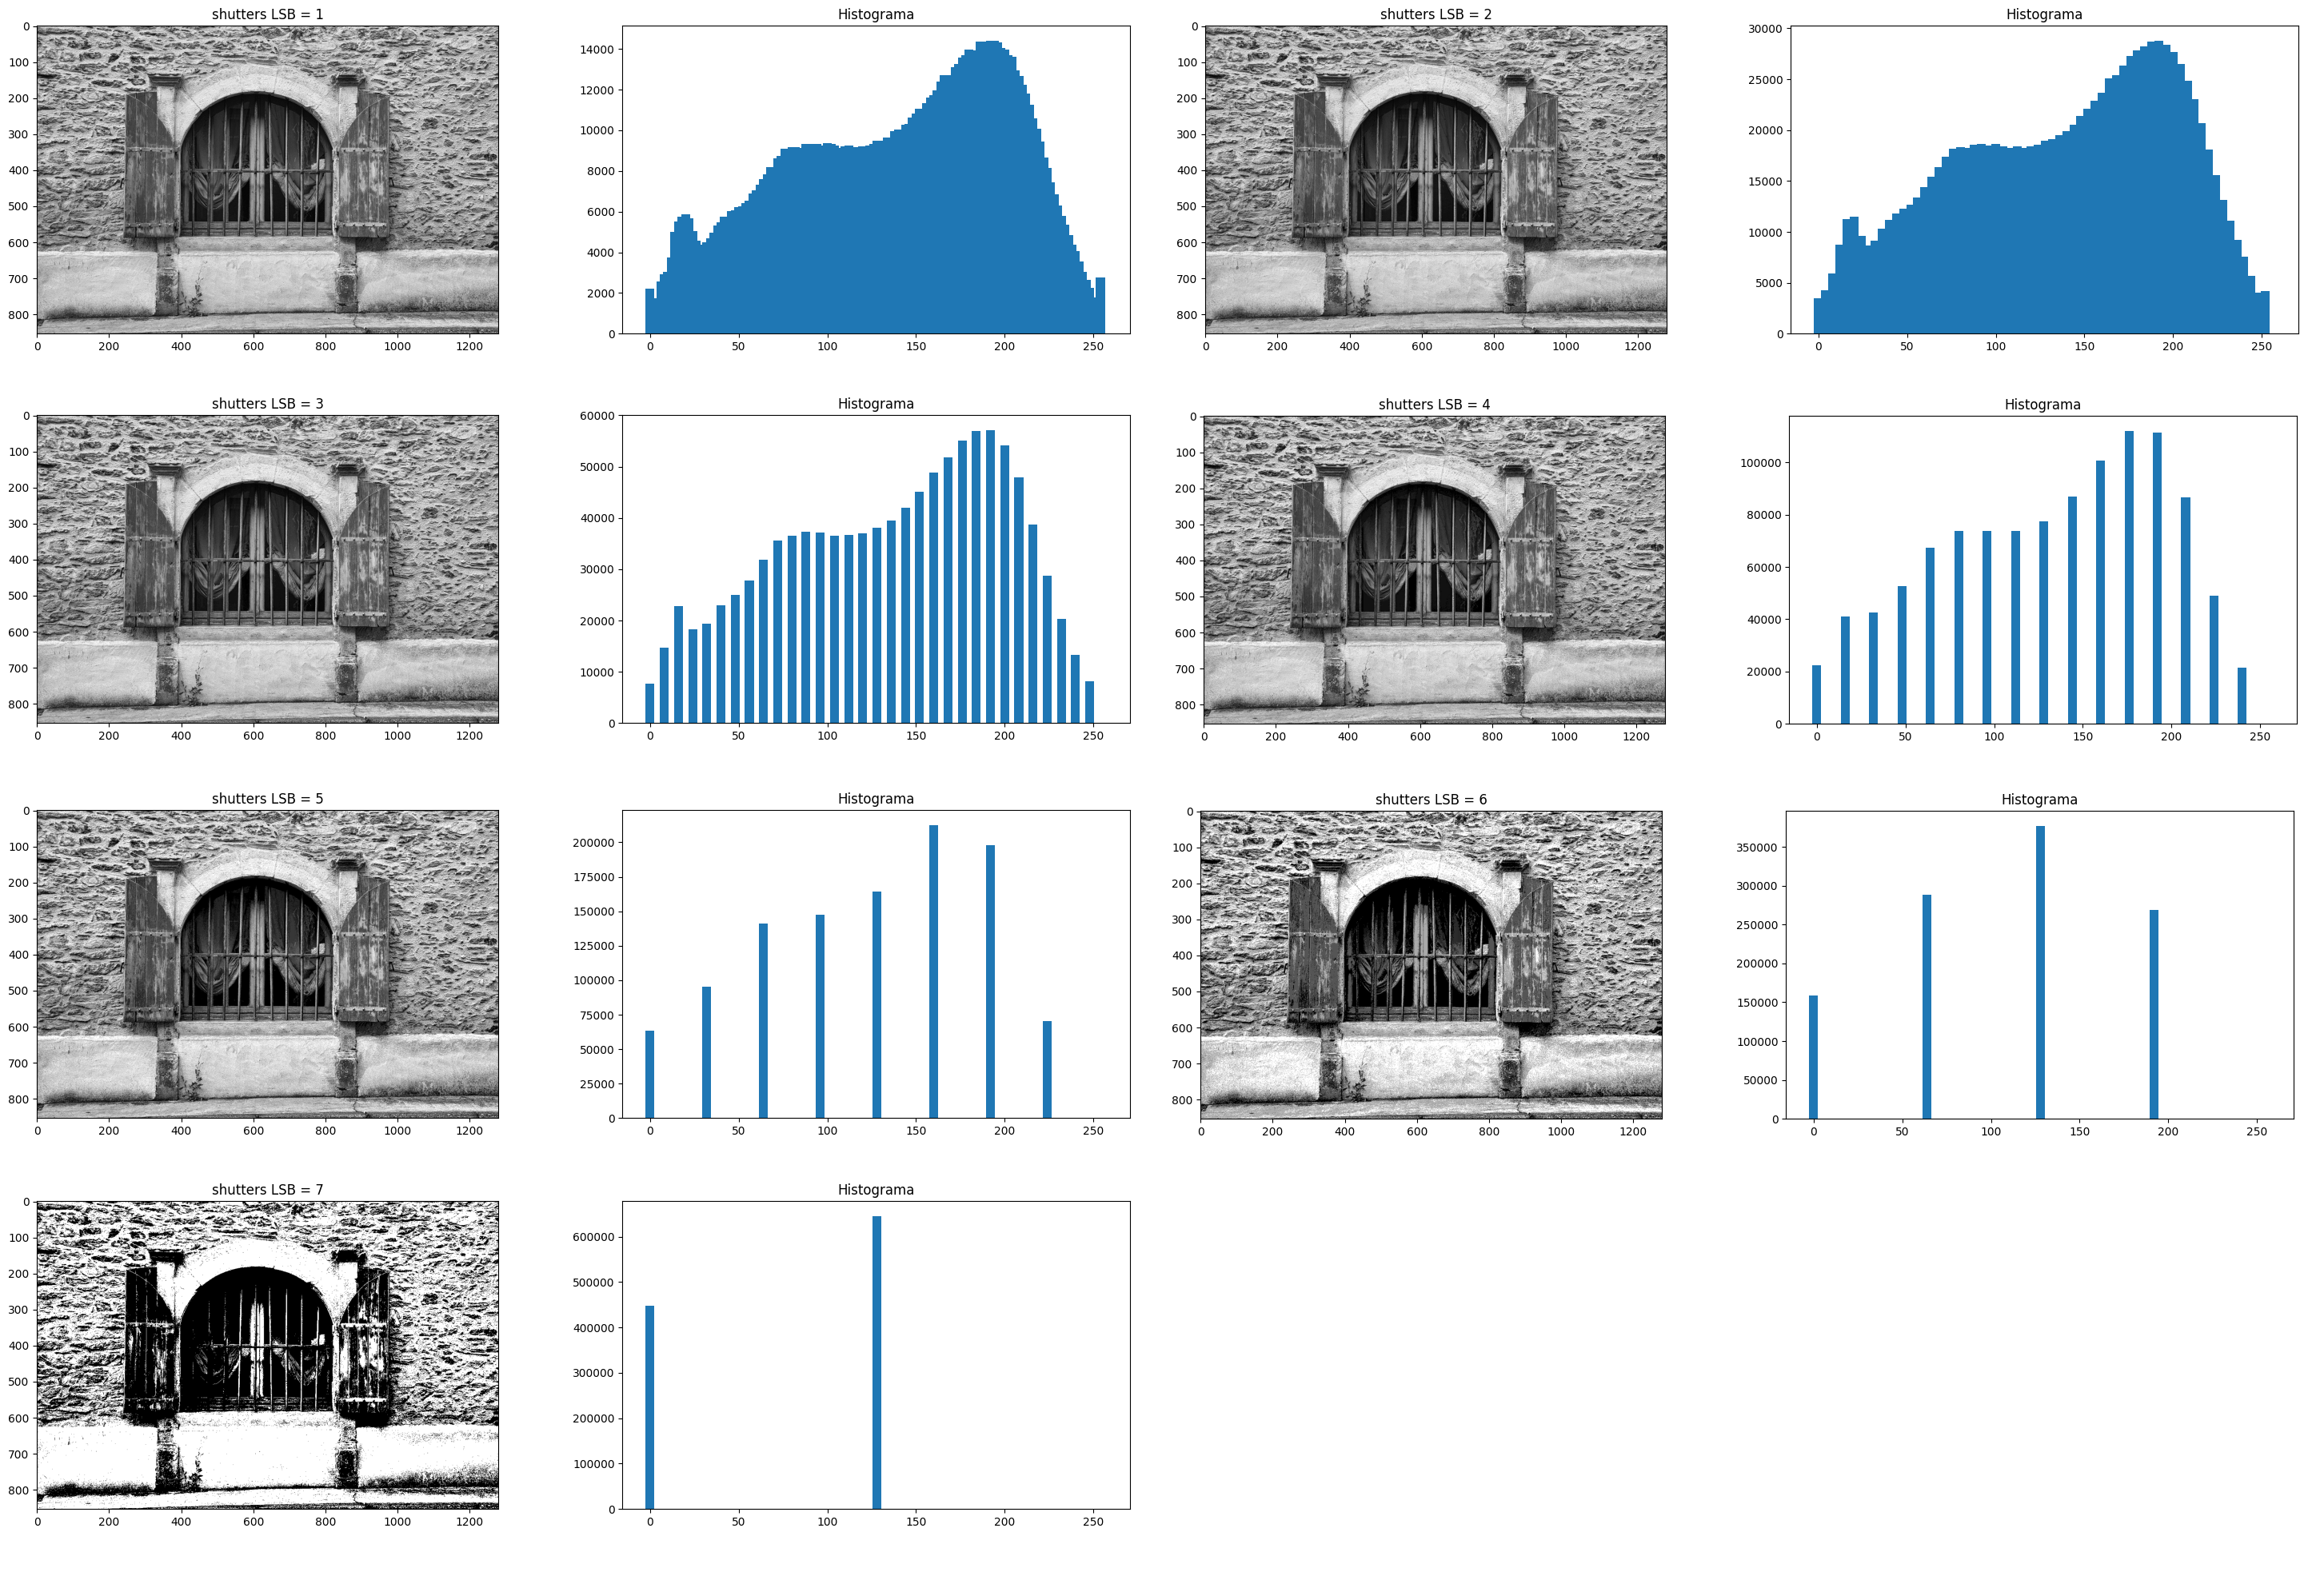
\includegraphics[scale=0.16]{Imagens/resultados-shutters-lsb.png}
    \end{figure}  
\end{frame}

\begin{frame}{Resultados - LSB}
    \begin{figure}
        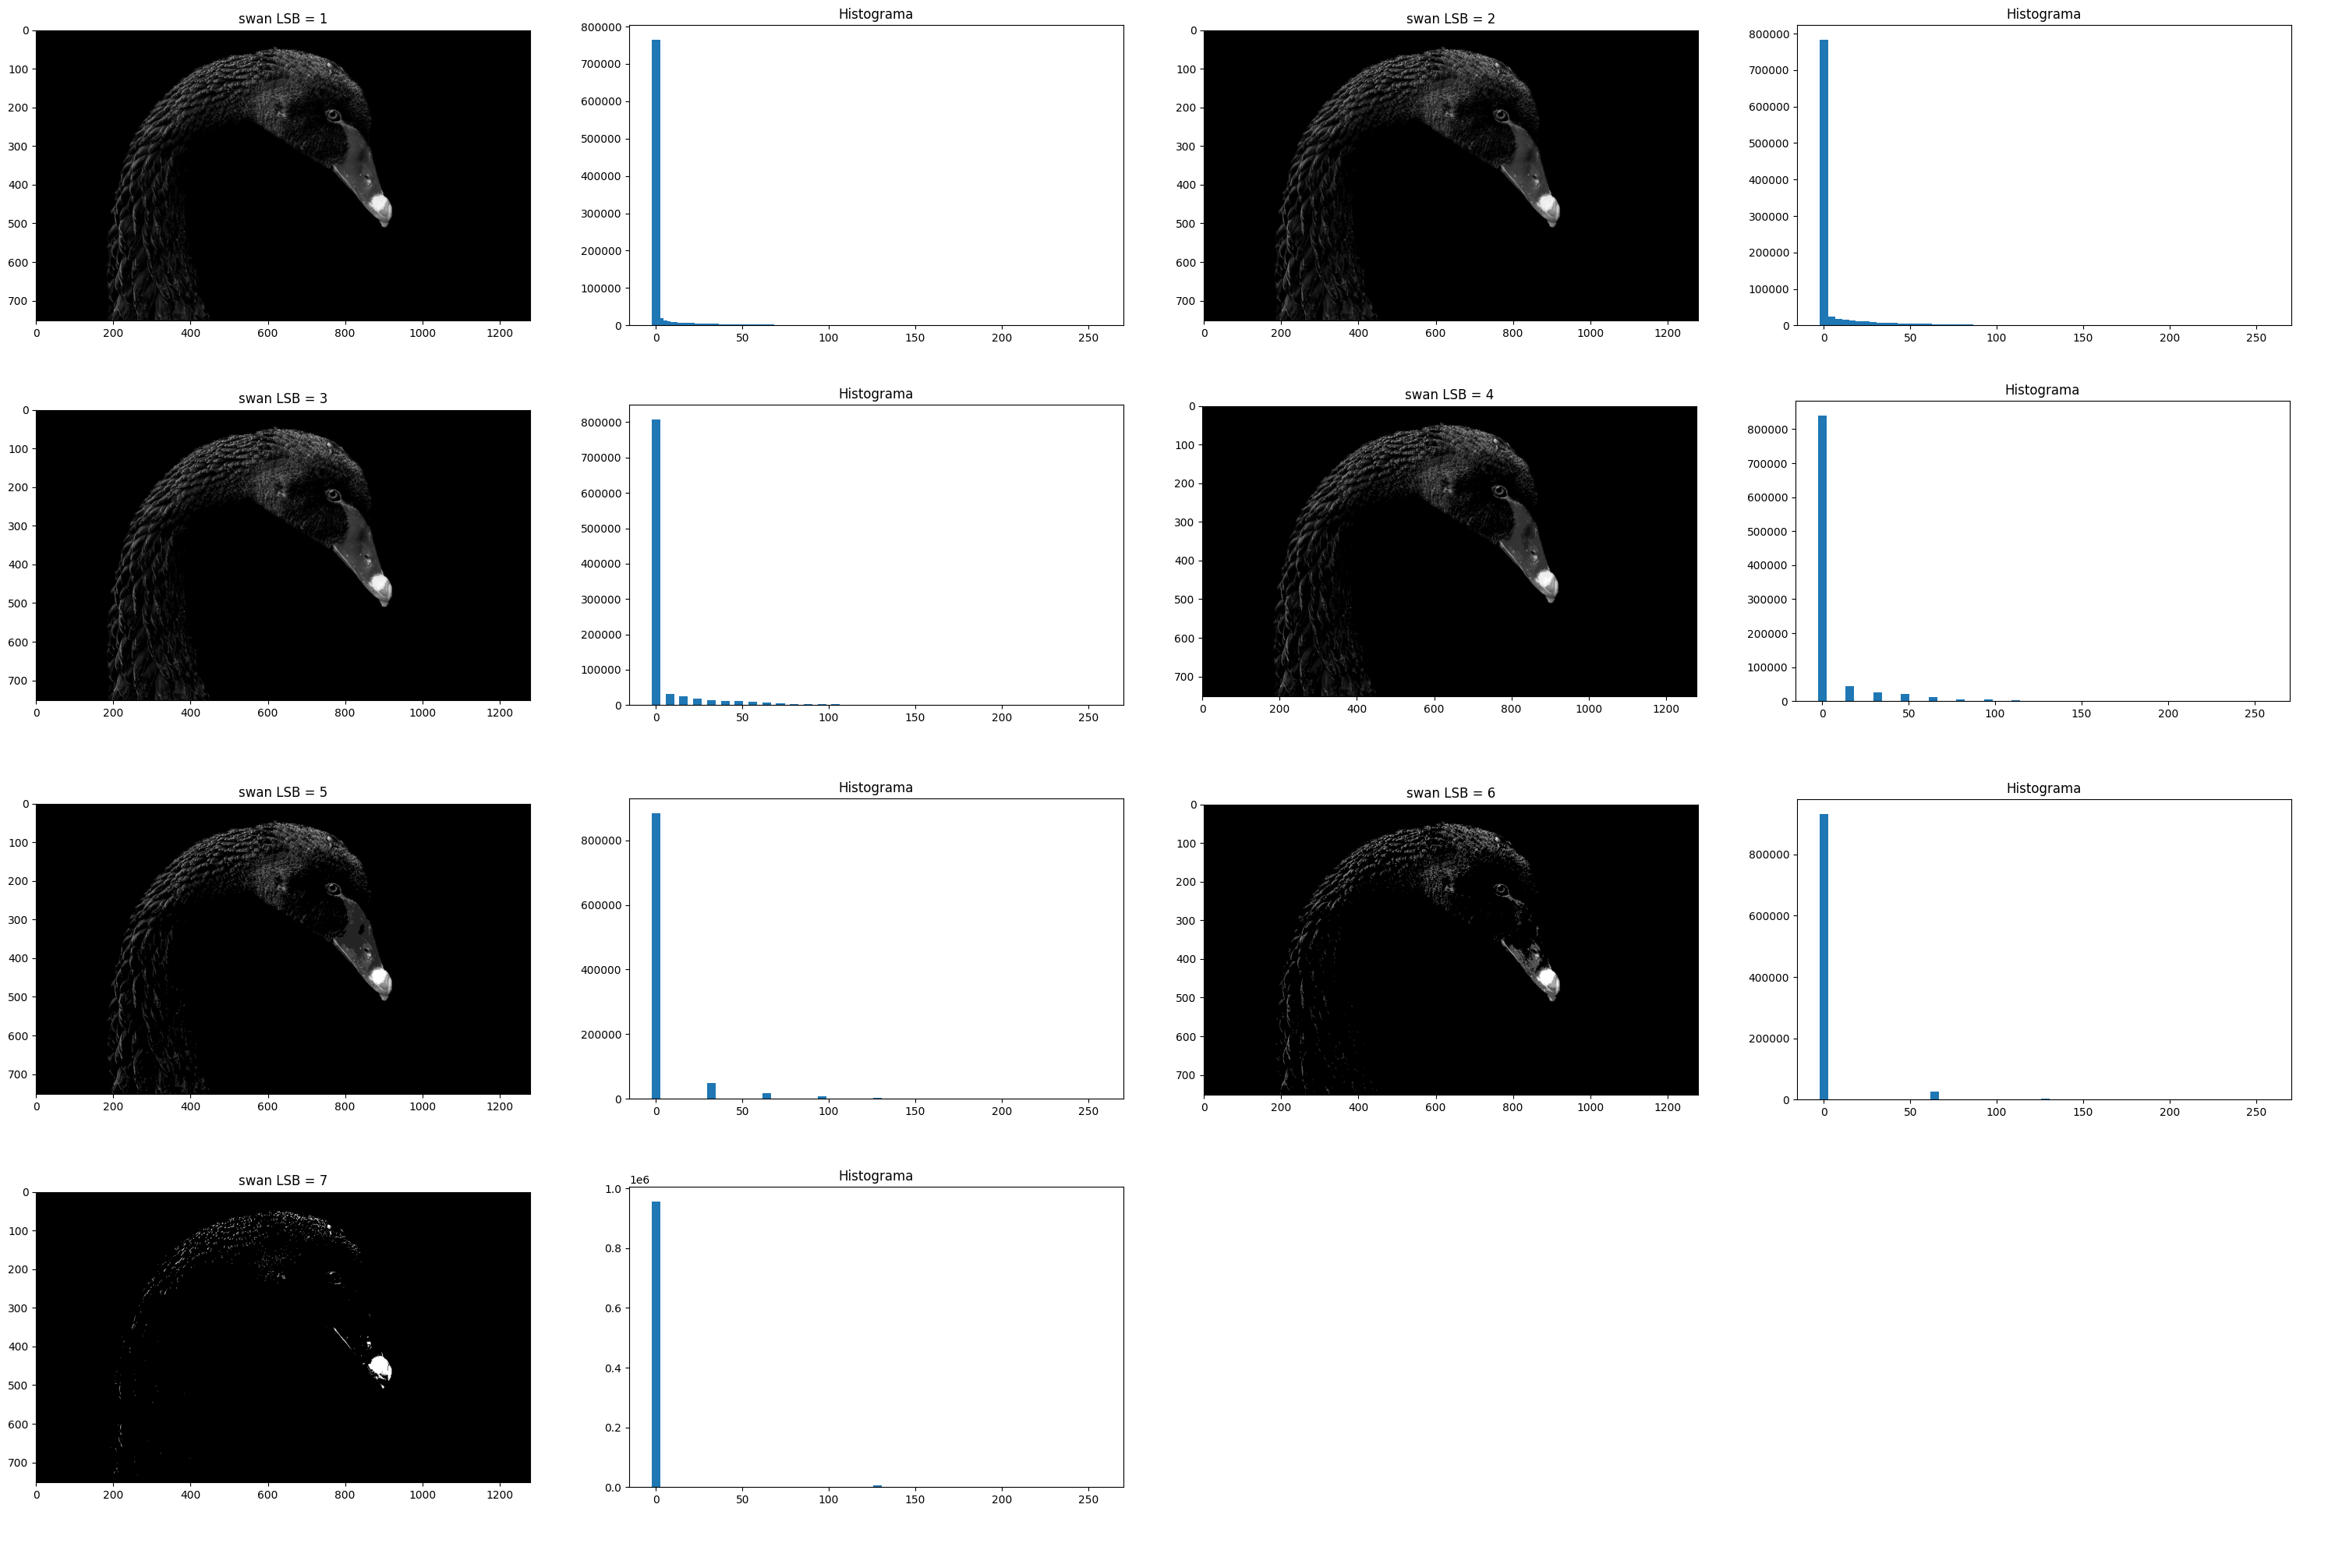
\includegraphics[scale=0.16]{Imagens/resultados-swan-lsb.png}
    \end{figure}  
\end{frame}

\begin{frame}{Resultados - MSB}
    \begin{figure}
        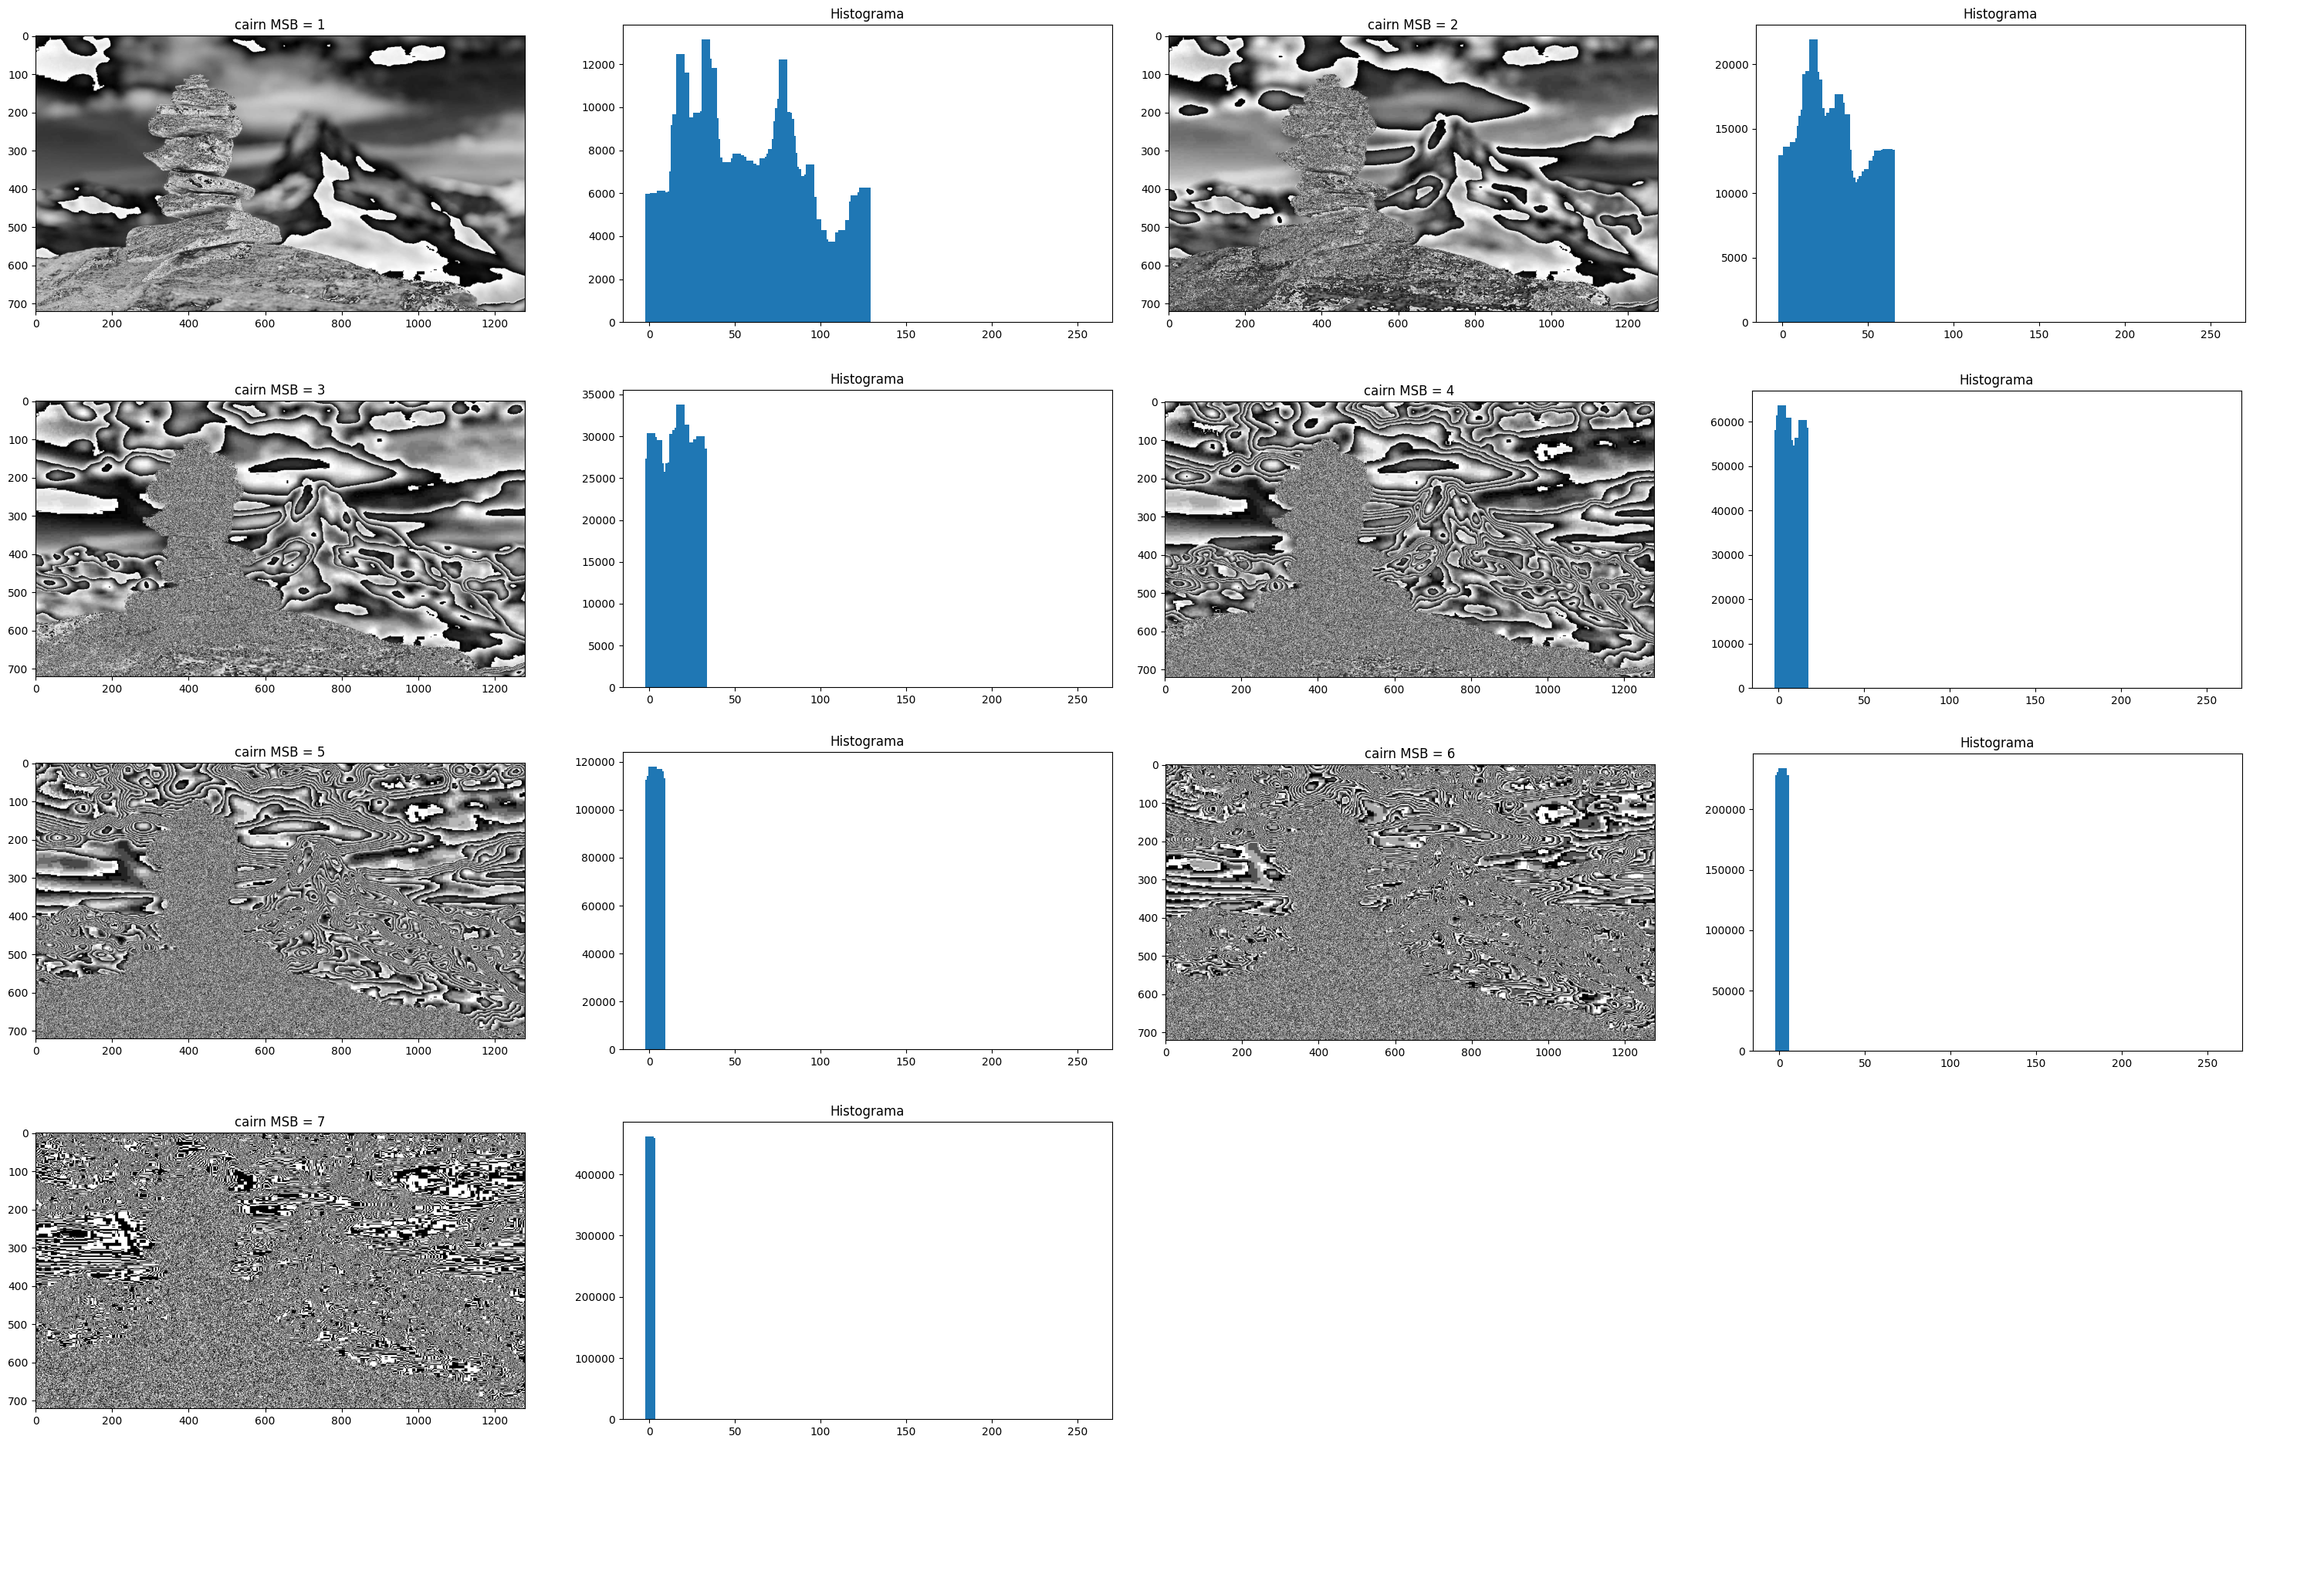
\includegraphics[scale=0.16]{Imagens/resultados-cairn-msb.png}
    \end{figure}  
\end{frame}

\begin{frame}{Resultados - MSB}
    \begin{figure}
        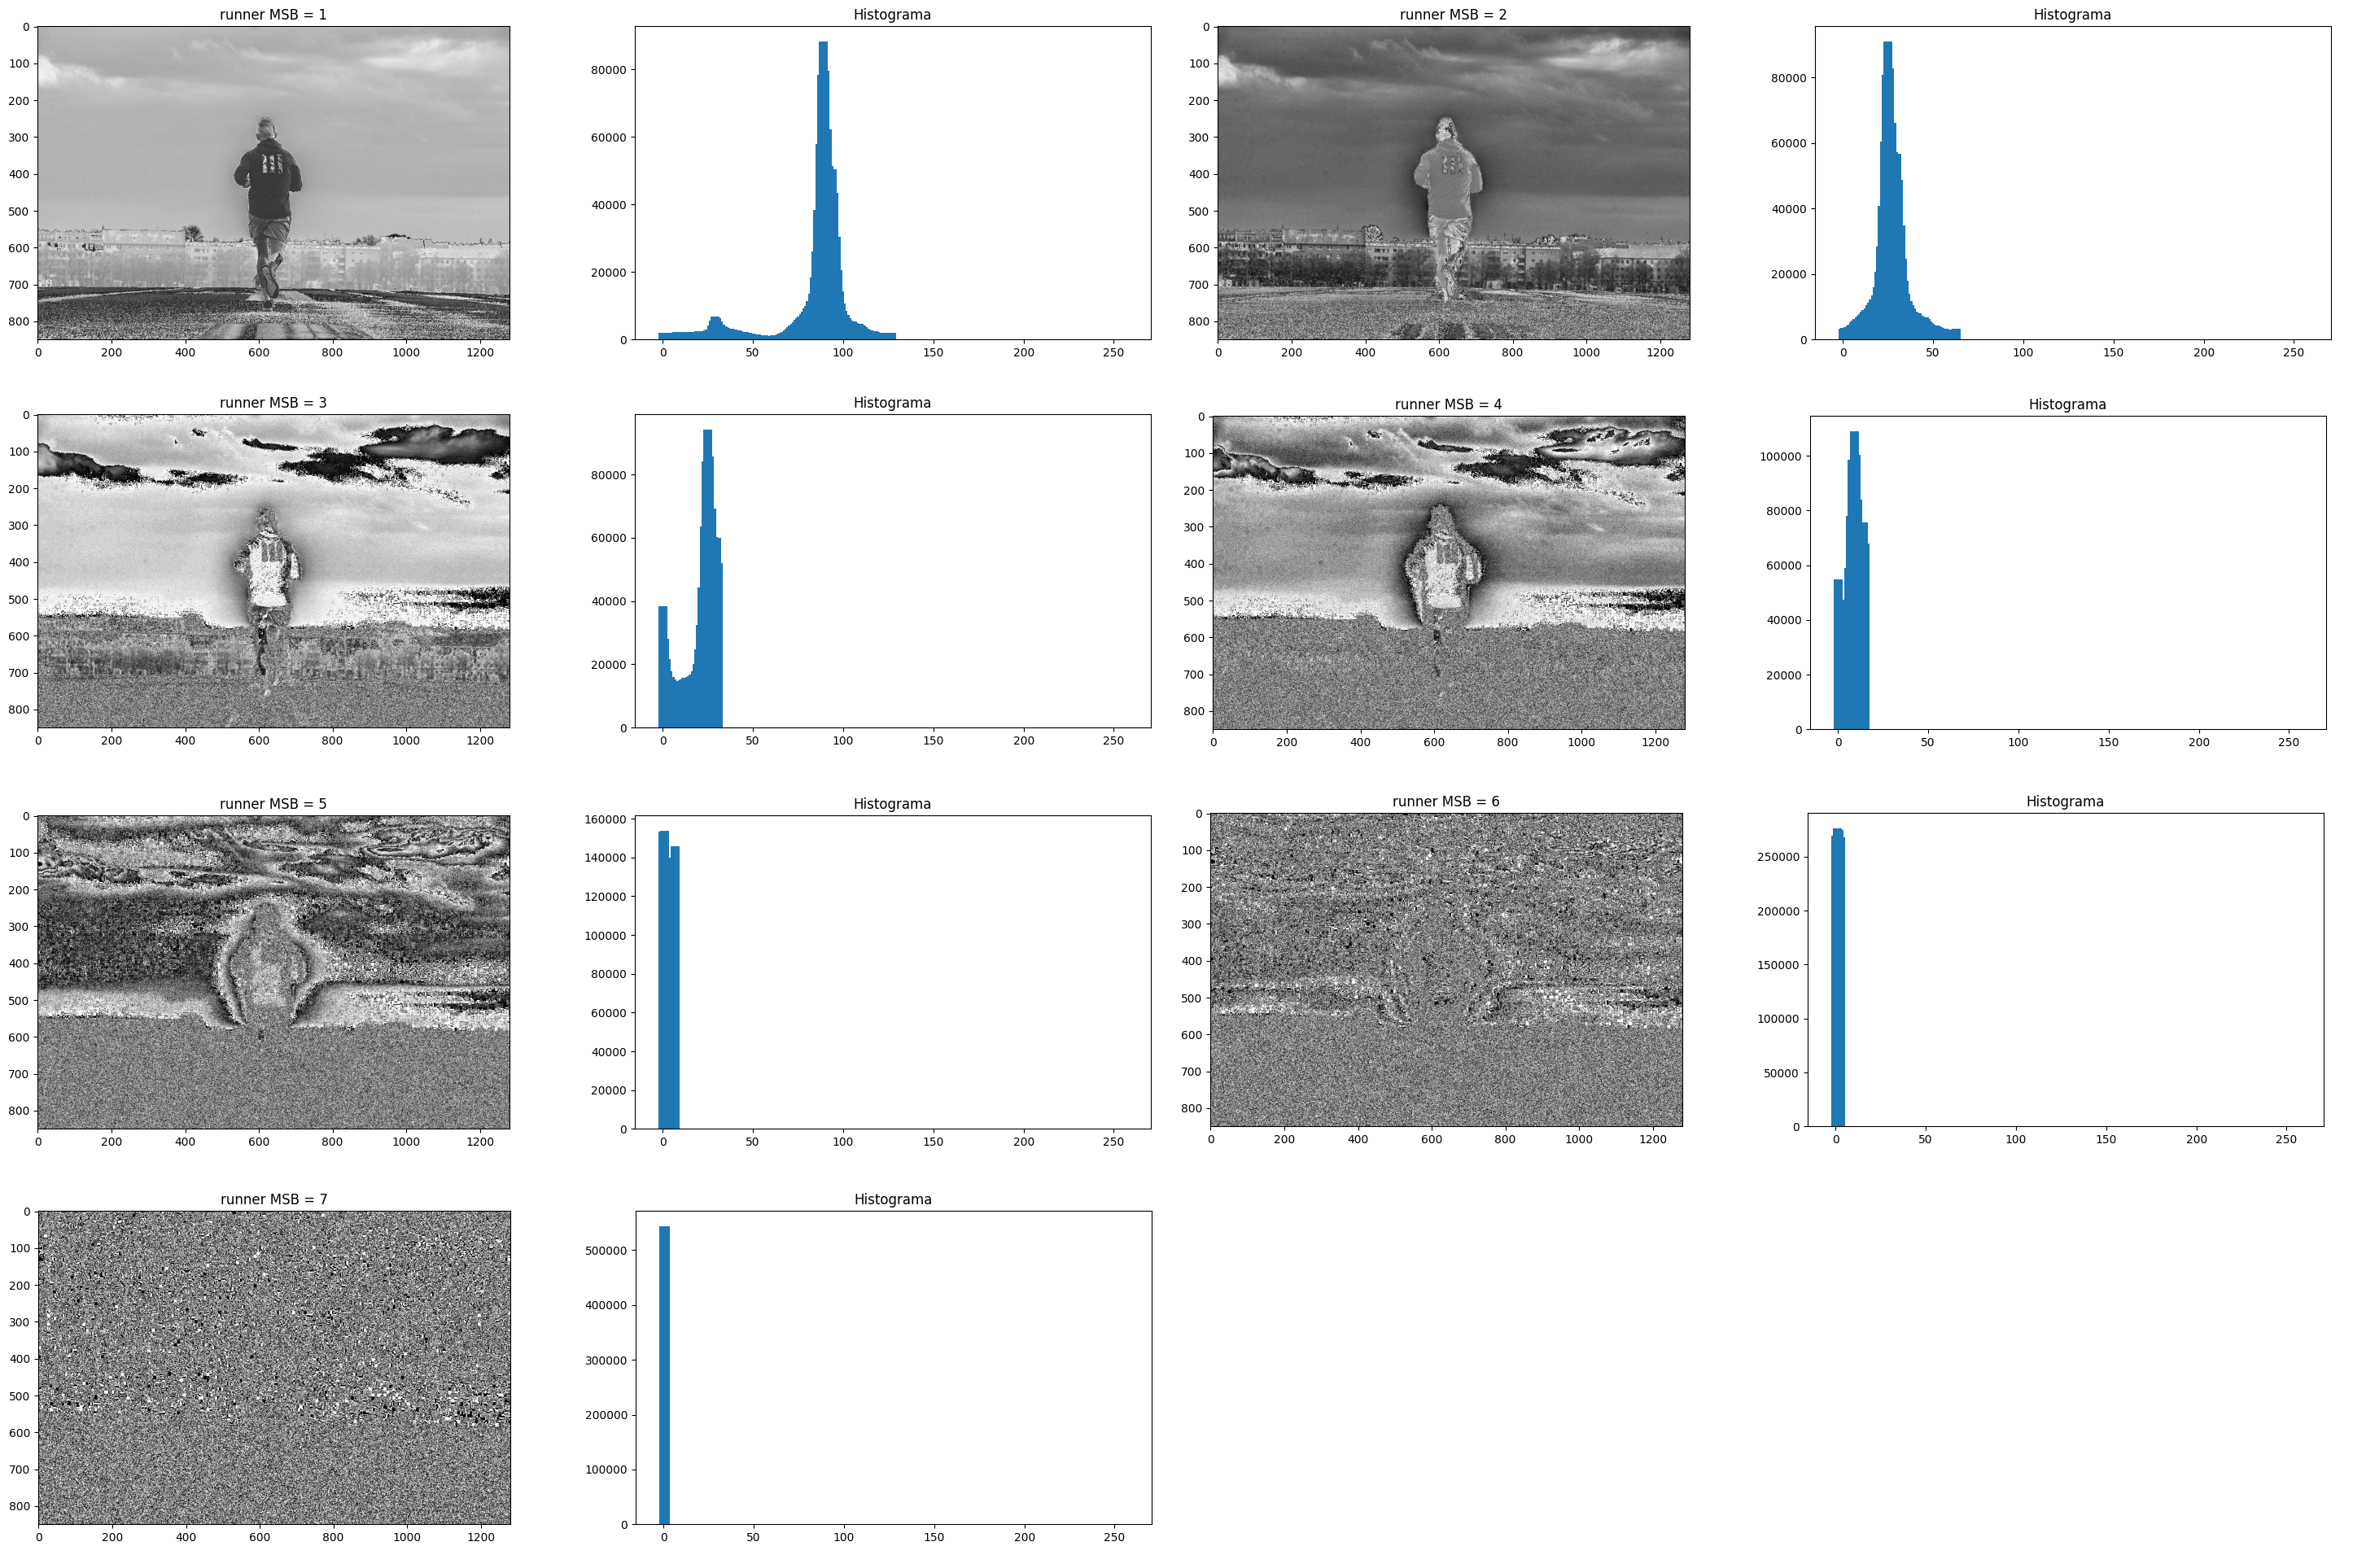
\includegraphics[scale=0.16]{Imagens/resultados-runner-msb.png}
    \end{figure}  
\end{frame}

\begin{frame}{Resultados - MSB}
    \begin{figure}
        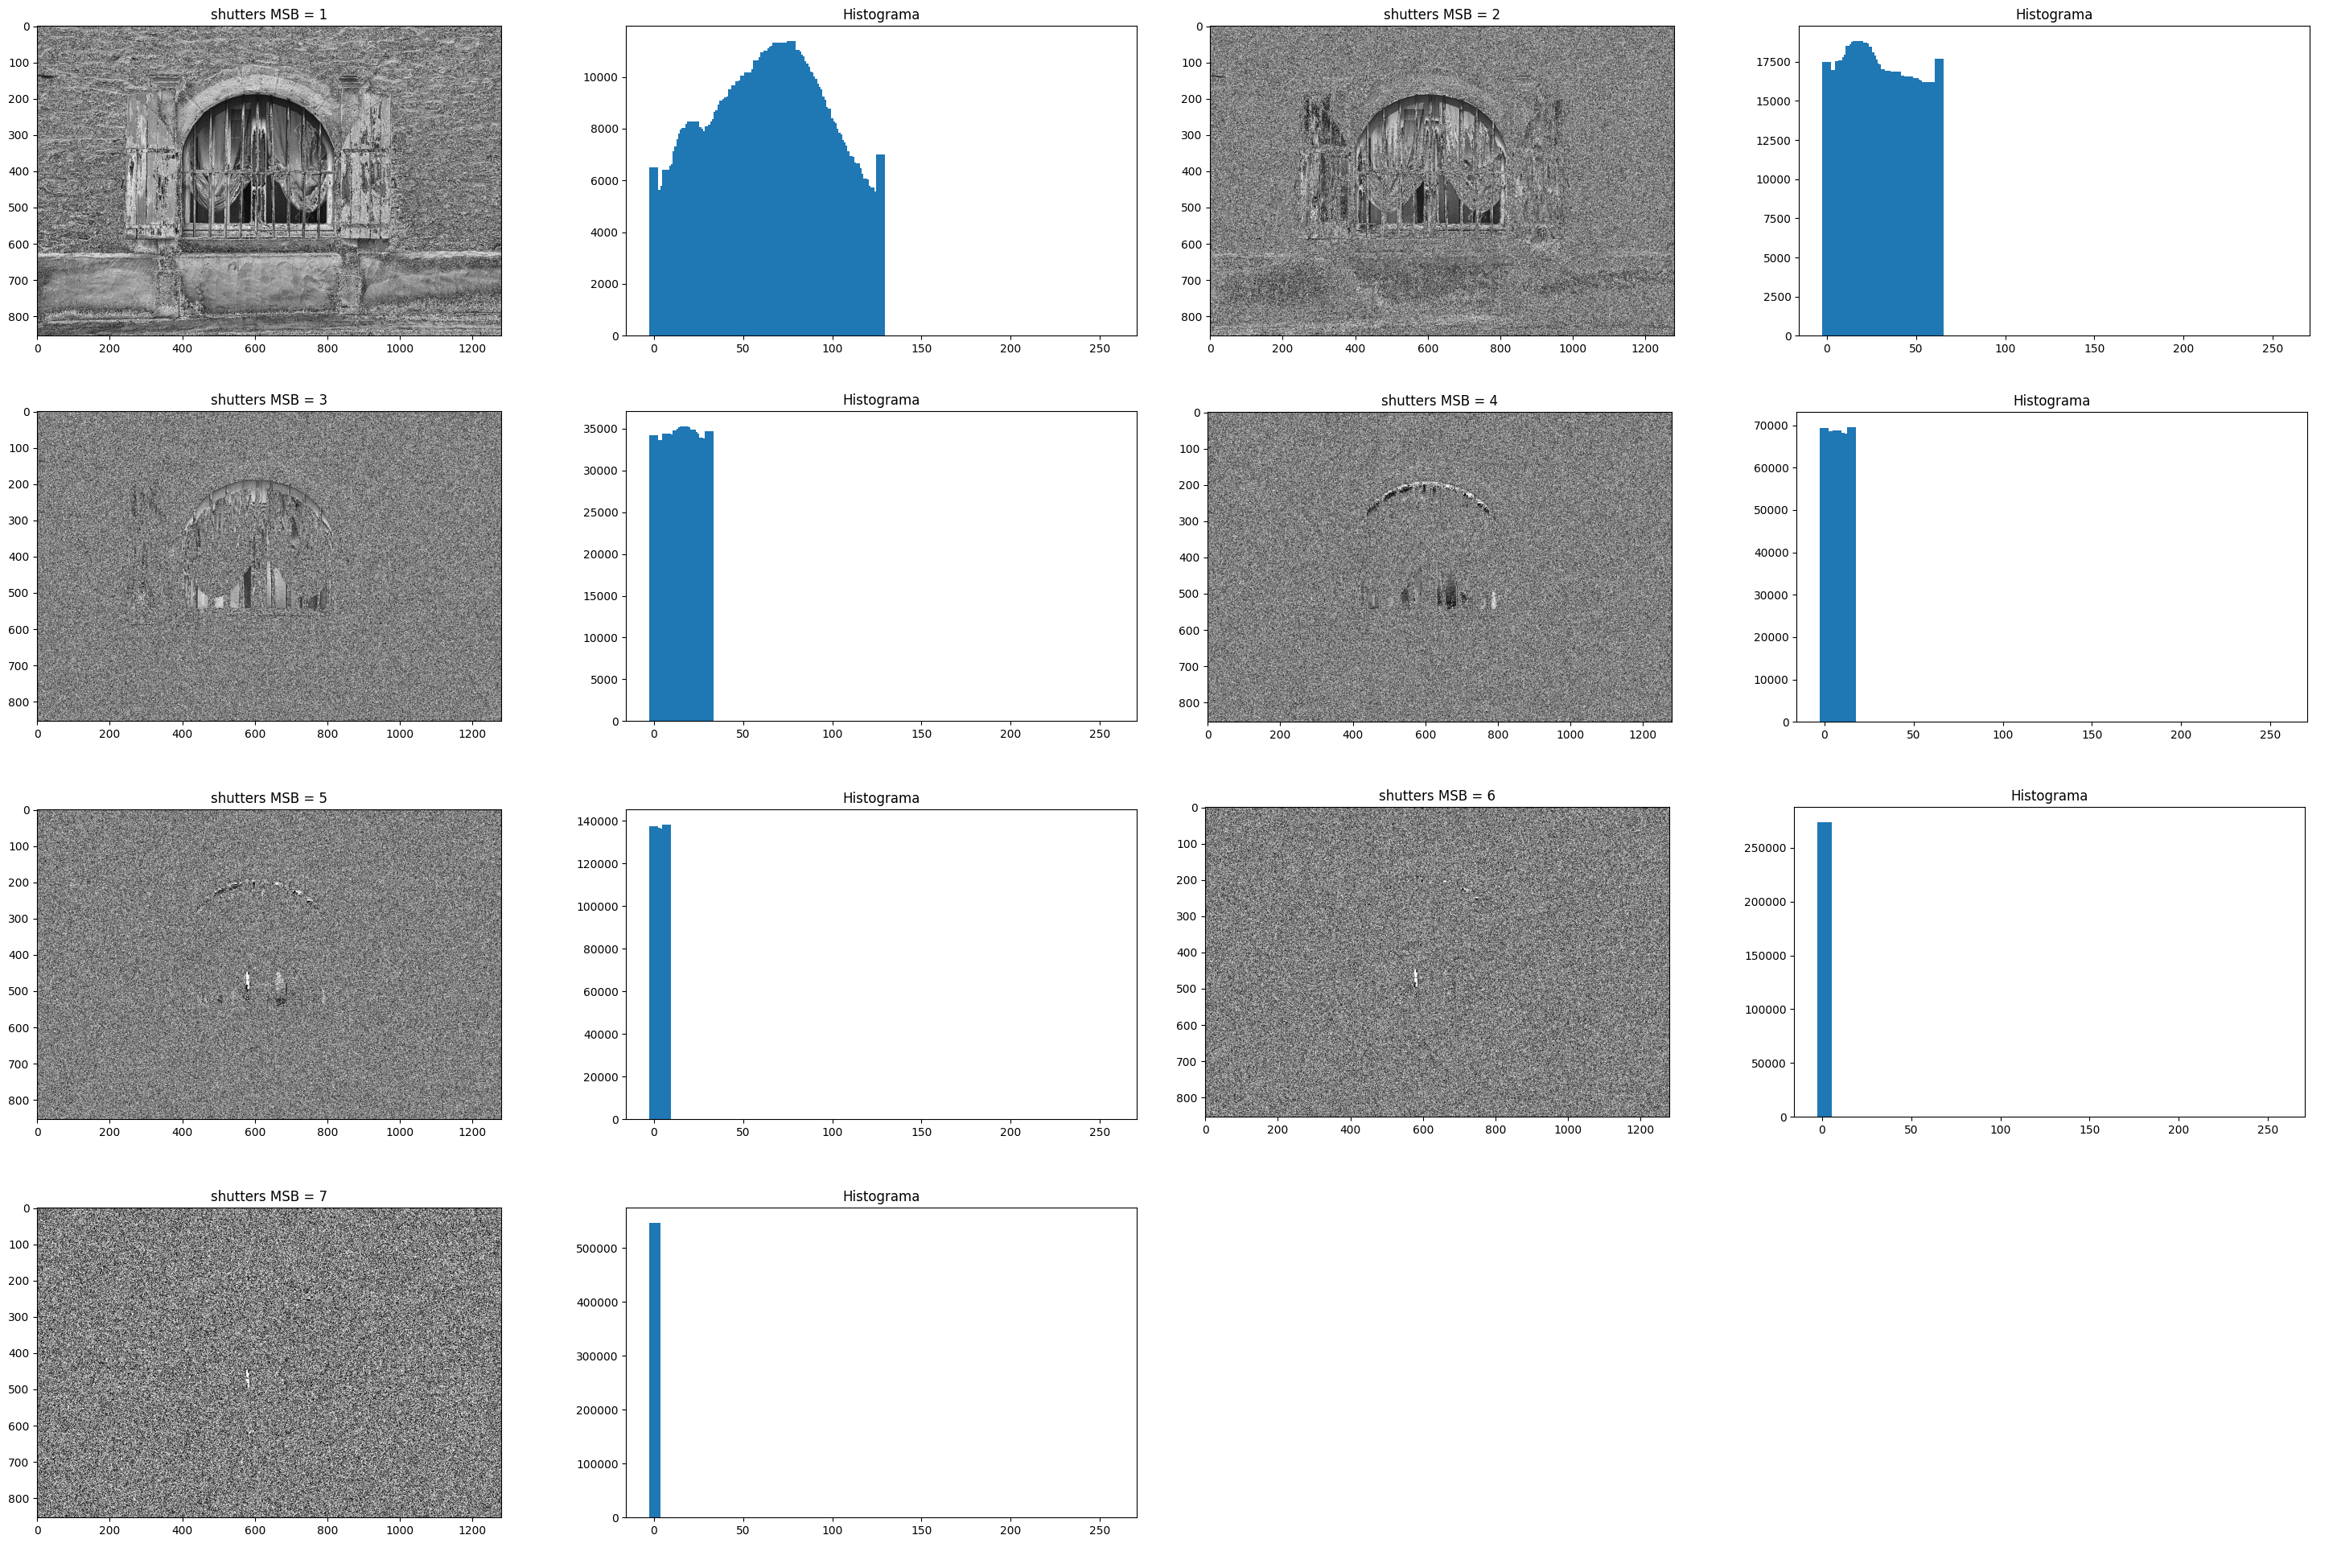
\includegraphics[scale=0.16]{Imagens/resultados-shutters-msb.png}
    \end{figure}  
\end{frame}

\begin{frame}{Resultados - MSB}
    \begin{figure}
        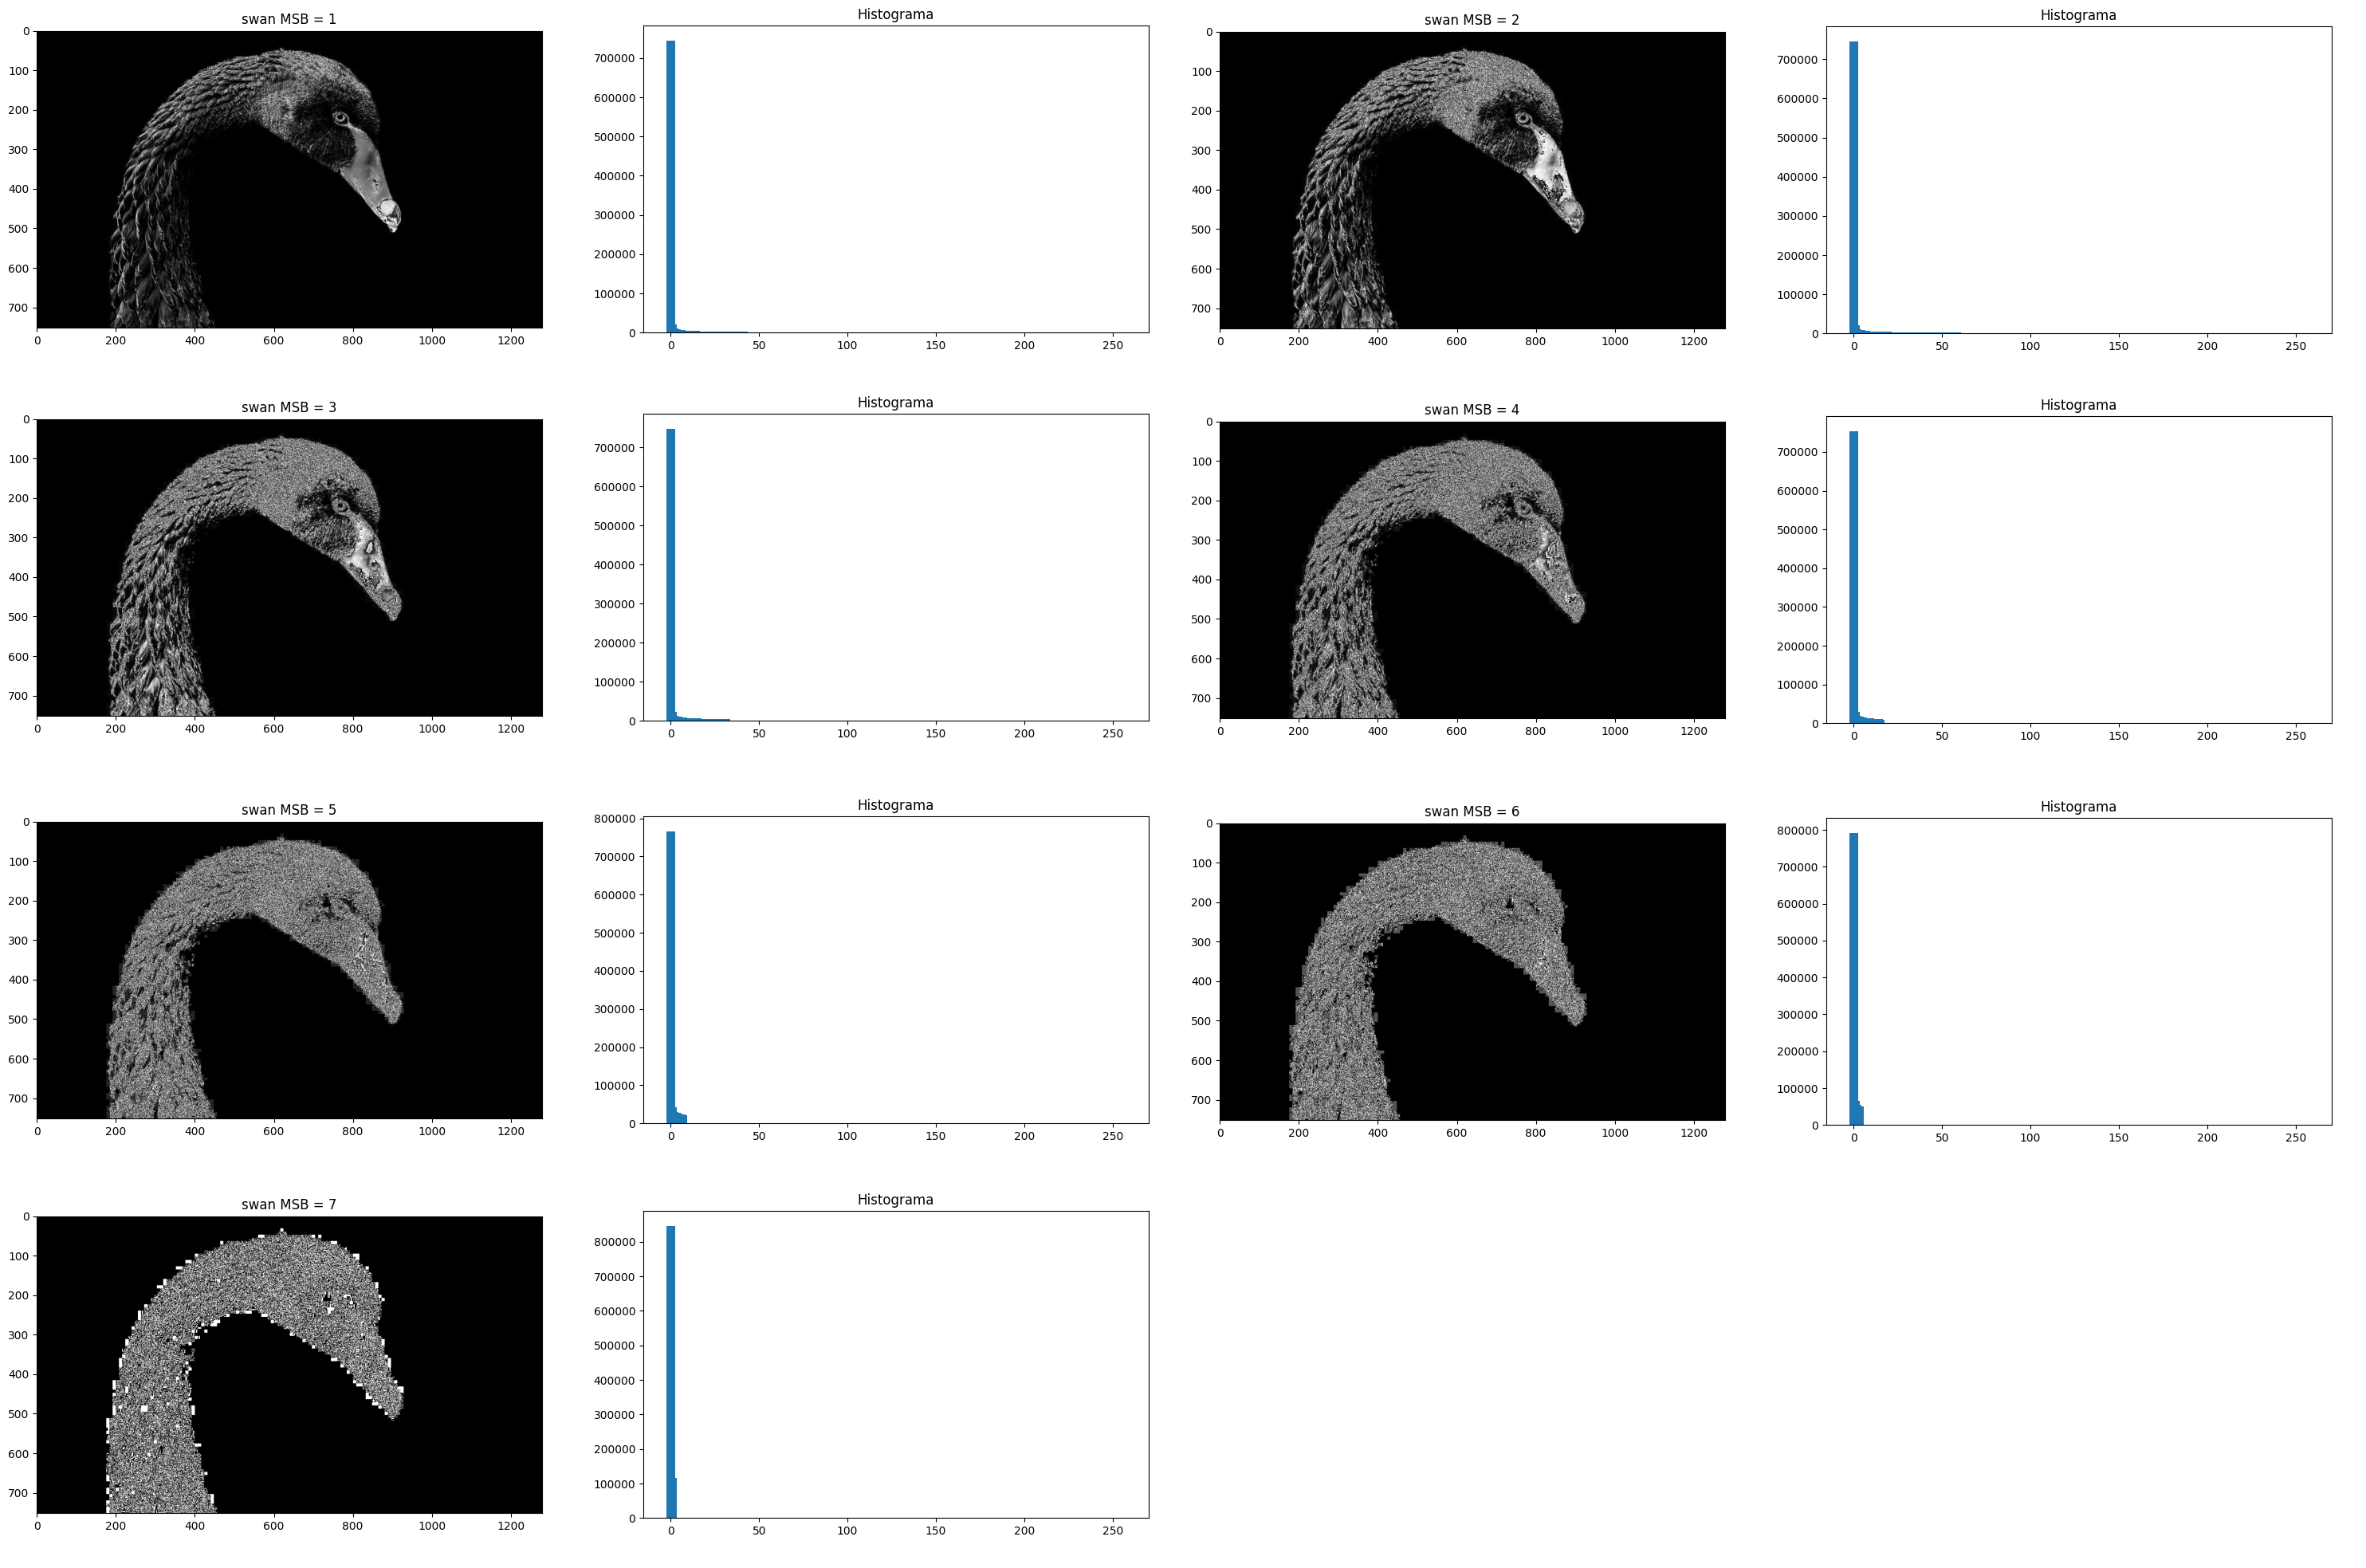
\includegraphics[scale=0.16]{Imagens/resultados-swan-msb.png}
    \end{figure}  
\end{frame}

\section{Conclusão}


\begin{frame}{Resultados - LSB/MSB}
\begin{table}[h!]
\centering
\begingroup
\tiny
\begin{tabular}{ccccccccc}
\hline
& \multicolumn{2}{c}{cairn} & \multicolumn{2}{c}{runner} & \multicolumn{2}{c}{shutters} & \multicolumn{2}{c}{swan} \\
& PSNR & SSIM & PSNR & SSIM & PSNR & SSIM & PSNR & SSIM \\
\hline
LSB 1 & 51.1575 & 0.9974 & 51.1388 & 0.9971 & 51.1370 & 0.9997 & 57.3143 & 0.9985 \\
LSB 2 & 42.6962 & 0.9881 & 42.7157 & 0.9862 & 42.6864 & 0.9985 & 49.3048 & 0.9943 \\
LSB 3 & 35.6999 & 0.9601 & 35.7731 & 0.9508 & 35.6897 & 0.9935 & 42.6692 & 0.9811 \\
LSB 4 & 29.3002 & 0.9016 & 28.6152 & 0.9076 & 29.2425 & 0.9745 & 36.6770 & 0.9489 \\
LSB 5 & 22.9212 & 0.8368 & 21.1971 & 0.7985 & 23.0121 & 0.9097 & 30.9843 & 0.8891 \\
LSB 6 & 17.2683 & 0.7523 & 18.8059 & 0.7843 & 17.0194 & 0.7504 & 25.9452 & 0.8202 \\
LSB 7 & 11.5796 & 0.5277 & 9.4766 & 0.5577 & 11.0111 & 0.3688 & 22.6162 & 0.7695 \\
\hline
MSB 1 & 6.9259 & 0.4390 & 7.1952 & 0.6076 & 8.2724 & 0.2938 & 28.5954 & 0.9780 \\
MSB 2 & 5.2902 & 0.2337 & 3.8795 & 0.2474 & 6.1461 & 0.0507 & 24.5492 & 0.9166 \\
MSB 3 & 4.5613 & 0.1089 & 3.5696 & 0.1169 & 5.2922 & 0.0205 & 22.8298 & 0.8587 \\
MSB 4 & 4.1211 & 0.0347 & 2.9918 & 0.0351 & 4.8618 & 0.0030 & 21.9574 & 0.8102 \\
MSB 5 & 3.9201 & 0.0099 & 2.7581 & 0.0037 & 4.6506 & 0.0003 & 21.5006 & 0.7812 \\
MSB 6 & 3.8171 & 0.0018 & 2.6761 & 0.0007 & 4.5456 & 0.0000 & 21.2674 & 0.7628 \\
MSB 7 & 3.7659 & 0.0001 & 2.6324 & 0.0000 & 4.4935 & 0.0000 & 21.1479 & 0.7510 \\
\hline
\end{tabular}
\endgroup
\end{table} 
\end{frame}

\begin{frame}{Resultados - LSB/MSB}
\begin{figure}
    \begin{tabular}{cc}
         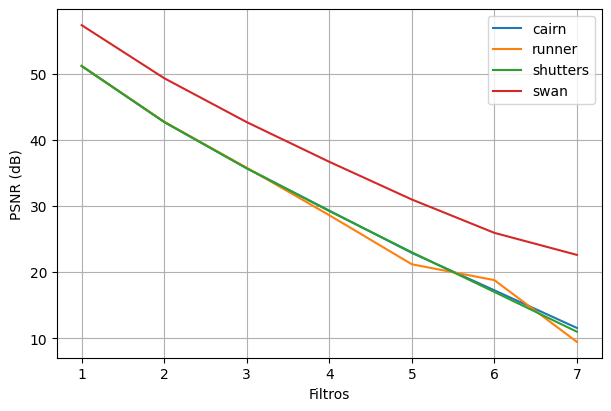
\includegraphics[scale=0.3]{Imagens/resultados-lsb-psnr.png} &   
         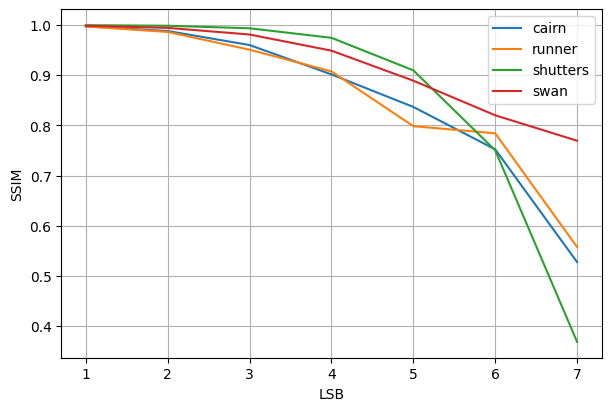
\includegraphics[scale=0.3]{Imagens/resultados-lsb-ssim.png} \\
         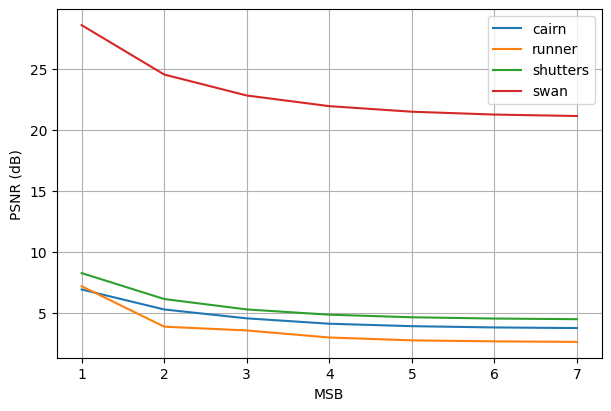
\includegraphics[scale=0.3]{Imagens/resultados-msb-psnr.png} &   
         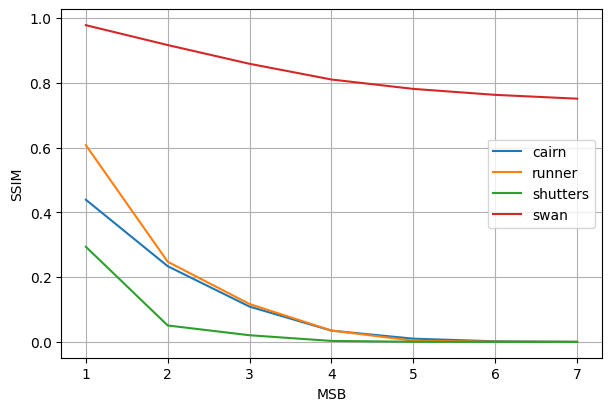
\includegraphics[scale=0.3]{Imagens/resultados-msb-ssim.png} \\
    \end{tabular}
\end{figure}
\end{frame}

\begin{frame}{Conclusão}

\begin{itemize}
    \item Importância do Histograma;
    \item Imagens com maior contraste -> Dificuldade de correção/binarização;
    \item Zerar MSBs em Regiões escuras -> Poucos ruídos;
    \item Mais informação espacial -> Mais LSBs.
\end{itemize}

\end{frame}


\end{document}